%  A simple AAU report template.
%  2015-05-08 v. 1.2.0
%  Copyright 2010-2015 by Jesper Kjær Nielsen <jkn@es.aau.dk>
%
%  This is free software: you can redistribute it and/or modify
%  it under the terms of the GNU General Public License as published by
%  the Free Software Foundation, either version 3 of the License, or
%  (at your option) any later version.
%
%  This is distributed in the hope that it will be useful,
%  but WITHOUT ANY WARRANTY; without even the implied warranty of
%  MERCHANTABILITY or FITNESS FOR A PARTICULAR PURPOSE.  See the
%  GNU General Public License for more details.
%
%  You can find the GNU General Public License at <http://www.gnu.org/licenses/>.
%
%  A simple AAU report template.
%  2015-05-08 v. 1.2.0
%  Copyright 2010-2015 by Jesper Kjær Nielsen <jkn@es.aau.dk>
%
%  This is free software: you can redistribute it and/or modify
%  it under the terms of the GNU General Public License as published by
%  the Free Software Foundation, either version 3 of the License, or
%  (at your option) any later version.
%
%  This is distributed in the hope that it will be useful,
%  but WITHOUT ANY WARRANTY; without even the implied warranty of
%  MERCHANTABILITY or FITNESS FOR A PARTICULAR PURPOSE.  See the
%  GNU General Public License for more details.
%
%  You can find the GNU General Public License at <http://www.gnu.org/licenses/>.
%
\documentclass[11pt,twoside,a4paper,openright]{report}
%%%%%%%%%%%%%%%%%%%%%%%%%%%%%%%%%%%%%%%%%%%%%%%%
% Language, Encoding and Fonts
% http://en.wikibooks.org/wiki/LaTeX/Internationalization
%%%%%%%%%%%%%%%%%%%%%%%%%%%%%%%%%%%%%%%%%%%%%%%%
% Select encoding of your inputs. Depends on
% your operating system and its default input
% encoding. Typically, you should use
%   Linux  : utf8 (most modern Linux distributions)
%            latin1 
%   Windows: ansinew
%            latin1 (works in most cases)
%   Mac    : applemac
% Notice that you can manually change the input
% encoding of your files by selecting "save as"
% an select the desired input encoding. 
\usepackage[utf8]{inputenc}
% Make latex understand and use the typographic
% rules of the language used in the document.
\usepackage[danish,english]{babel}
% Choose the font encoding
\usepackage[T1]{fontenc}
%%%%%%%%%%%%%%%%%%%%%%%%%%%%%%%%%%%%%%%%%%%%%%%%
% Graphics and Tables
% http://en.wikibooks.org/wiki/LaTeX/Importing_Graphics
% http://en.wikibooks.org/wiki/LaTeX/Tables
% http://en.wikibooks.org/wiki/LaTeX/Colors
%%%%%%%%%%%%%%%%%%%%%%%%%%%%%%%%%%%%%%%%%%%%%%%%
% load a colour package
\usepackage{xcolor}
\definecolor{aaublue}{RGB}{33,26,82}% dark blue
% The standard graphics inclusion package
\usepackage{graphicx}
\graphicspath{{./figures/}}
% Set up how figure and table captions are displayed
\usepackage{caption}
\captionsetup{%
  font=footnotesize,% set font size to footnotesize
  labelfont=bf % bold label (e.g., Figure 3.2) font
}
% Make the standard latex tables look so much better
\usepackage{array,booktabs}
% Enable the use of frames around, e.g., theorems
% The framed package is used in the example environment
\usepackage{framed}

%%%%%%%%%%%%%%%%%%%%%%%%%%%%%%%%%%%%%%%%%%%%%%%%
% Mathematics
% http://en.wikibooks.org/wiki/LaTeX/Mathematics
%%%%%%%%%%%%%%%%%%%%%%%%%%%%%%%%%%%%%%%%%%%%%%%%
% Defines new environments such as equation,
% align and split 
\usepackage{amsmath}
\usepackage{subcaption}
% Adds new math symbols
\usepackage{amssymb}
\usepackage[figure]{algorithm2e}
% Use theorems in your document
% The ntheorem package is also used for the example environment
% When using thmmarks, amsmath must be an option as well. Otherwise \eqref doesn't work anymore.
\usepackage[framed,amsmath,thmmarks]{ntheorem}

%%%%%%%%%%%%%%%%%%%%%%%%%%%%%%%%%%%%%%%%%%%%%%%%
% Page Layout
% http://en.wikibooks.org/wiki/LaTeX/Page_Layout
%%%%%%%%%%%%%%%%%%%%%%%%%%%%%%%%%%%%%%%%%%%%%%%%
% Change margins, papersize, etc of the document
\usepackage[
  inner=28mm,% left margin on an odd page
  outer=41mm,% right margin on an odd page
  ]{geometry}
% Modify how \chapter, \section, etc. look
% The titlesec package is very configureable
\usepackage{titlesec}
\titleformat{\chapter}[display]{\normalfont\huge\bfseries}{\chaptertitlename\ \thechapter}{20pt}{\Huge}
\titleformat*{\section}{\normalfont\Large\bfseries}
\titleformat*{\subsection}{\normalfont\large\bfseries}
\titleformat*{\subsubsection}{\normalfont\normalsize\bfseries}
%\titleformat*{\paragraph}{\normalfont\normalsize\bfseries}
%\titleformat*{\subparagraph}{\normalfont\normalsize\bfseries}

\usepackage{float}
% Clear empty pages between chapters
\let\origdoublepage\cleardoublepage
\newcommand{\clearemptydoublepage}{%
  \clearpage
  {\pagestyle{empty}\origdoublepage}%
}
\let\cleardoublepage\clearemptydoublepage

% Change the headers and footers
\usepackage{fancyhdr}
\pagestyle{fancy}
\fancyhf{} %delete everything
\renewcommand{\headrulewidth}{0pt} %remove the horizontal line in the header
\fancyhead[RE]{\small\nouppercase\leftmark} %even page - chapter title
\fancyhead[LO]{\small\nouppercase\rightmark} %uneven page - section title
\fancyhead[LE,RO]{\thepage} %page number on all pages
% Do not stretch the content of a page. Instead,
% insert white space at the bottom of the page
\raggedbottom
% Enable arithmetics with length. Useful when
% typesetting the layout.
\usepackage{calc}

%%%%%%%%%%%%%%%%%%%%%%%%%%%%%%%%%%%%%%%%%%%%%%%%
% Bibliography
% http://en.wikibooks.org/wiki/LaTeX/Bibliography_Management
%%%%%%%%%%%%%%%%%%%%%%%%%%%%%%%%%%%%%%%%%%%%%%%%
\usepackage[backend=bibtex,
  bibencoding=utf8,natbib
  ]{biblatex}
\addbibresource{bib/mybib}

%%%%%%%%%%%%%%%%%%%%%%%%%%%%%%%%%%%%%%%%%%%%%%%%
% Misc
%%%%%%%%%%%%%%%%%%%%%%%%%%%%%%%%%%%%%%%%%%%%%%%%
% Add bibliography and index to the table of
% contents
\usepackage[nottoc]{tocbibind}
% Add the command \pageref{LastPage} which refers to the
% page number of the last page
\usepackage{lastpage}
% Add todo notes in the margin of the document
\usepackage[
%  disable, %turn off todonotes
  colorinlistoftodos, %enable a coloured square in the list of todos
  textwidth=\marginparwidth, %set the width of the todonotes
  textsize=scriptsize, %size of the text in the todonotes
  ]{todonotes}

%%%%%%%%%%%%%%%%%%%%%%%%%%%%%%%%%%%%%%%%%%%%%%%%
% Hyperlinks
% http://en.wikibooks.org/wiki/LaTeX/Hyperlinks
%%%%%%%%%%%%%%%%%%%%%%%%%%%%%%%%%%%%%%%%%%%%%%%%
% Enable hyperlinks and insert info into the pdf
% file. Hypperref should be loaded as one of the 
% last packages
\usepackage{hyperref}
\hypersetup{%
	pdfpagelabels=true,%
	plainpages=false,%
	pdfauthor={Author(s)},%
	pdftitle={Title},%
	pdfsubject={Subject},%
	bookmarksnumbered=true,%
	colorlinks=true,%
	citecolor=black,%
	filecolor=black,%
	linkcolor=black,% you should probably change this to black before printing
	urlcolor=black,%
	pdfstartview=FitH%
}

\usepackage{cleveref}
\crefdefaultlabelformat{\textbf{#2#1#3}} % boldface only the number
% boldface only the type in front of the number
\crefname{figure}{\textbf{Figure}}{\textbf{Figures}}
\Crefname{figure}{\textbf{Figure}}{\textbf{Figures}}
% package inclusion and set up of the document
% see, e.g., http://en.wikibooks.org/wiki/LaTeX/Formatting#Hyphenation
% for more information on word hyphenation
\hyphenation{ex-am-ple hy-phen-a-tion short}
\hyphenation{long la-tex}
% 
%  A simple AAU report template.
%  2015-05-08 v. 1.2.0
%  Copyright 2010-2015 by Jesper Kjær Nielsen <jkn@es.aau.dk>
%
%  This is free software: you can redistribute it and/or modify
%  it under the terms of the GNU General Public License as published by
%  the Free Software Foundation, either version 3 of the License, or
%  (at your option) any later version.
%
%  This is distributed in the hope that it will be useful,
%  but WITHOUT ANY WARRANTY; without even the implied warranty of
%  MERCHANTABILITY or FITNESS FOR A PARTICULAR PURPOSE.  See the
%  GNU General Public License for more details.
%
%  You can find the GNU General Public License at <http://www.gnu.org/licenses/>.
%
%
%
% see, e.g., http://en.wikibooks.org/wiki/LaTeX/Customizing_LaTeX#New_commands
% for more information on how to create macros

%%%%%%%%%%%%%%%%%%%%%%%%%%%%%%%%%%%%%%%%%%%%%%%%
% Macros for the titlepage
%%%%%%%%%%%%%%%%%%%%%%%%%%%%%%%%%%%%%%%%%%%%%%%%
%Creates the aau titlepage
\newcommand{\aautitlepage}[3]{%
  {
    %set up various length
    \ifx\titlepageleftcolumnwidth\undefined
      \newlength{\titlepageleftcolumnwidth}
      \newlength{\titlepagerightcolumnwidth}
    \fi
    \setlength{\titlepageleftcolumnwidth}{0.5\textwidth-\tabcolsep}
    \setlength{\titlepagerightcolumnwidth}{\textwidth-2\tabcolsep-\titlepageleftcolumnwidth}
    %create title page
    \thispagestyle{empty}
    \noindent%
    \begin{tabular}{@{}ll@{}}
      \parbox{\titlepageleftcolumnwidth}{
        \iflanguage{danish}{%
          
\includegraphics[width=\titlepageleftcolumnwidth]{figures/aau_logo_da}
        }{%
          
\includegraphics[width=\titlepageleftcolumnwidth]{figures/aau_logo_en}
        }
      } &
      \parbox{\titlepagerightcolumnwidth}{\raggedleft\sf\small
        #2
      }\bigskip\\
       #1 &
      \parbox[t]{\titlepagerightcolumnwidth}{%
      \textbf{Abstract:}\bigskip\par
        \fbox{\parbox{\titlepagerightcolumnwidth-2\fboxsep-2\fboxrule}{%
          #3
        }}
      }\\
    \end{tabular}
    \vfill
    \iflanguage{danish}{%
      \noindent{\footnotesize\emph{Rapportens indhold er frit tilgængeligt, men offentliggørelse (med kildeangivelse) må kun ske efter aftale med forfatterne.}}
    }{%
      \noindent{\footnotesize\emph{The content of this report is freely available, but publication (with reference) may only be pursued due to agreement with the author.}}
    }
    \clearpage
  }
}

%Create english project info
\newcommand{\englishprojectinfo}[8]{%
  \parbox[t]{\titlepageleftcolumnwidth}{
    \textbf{Title:}\\ #1\bigskip\par
    \textbf{Theme:}\\ #2\bigskip\par
    \textbf{Project Period:}\\ #3\bigskip\par
    \textbf{Project Group:}\\ #4\bigskip\par
    \textbf{Participant(s):}\\ #5\bigskip\par
    \textbf{Supervisor(s):}\\ #6\bigskip\par
    \textbf{Copies:} #7\bigskip\par
    \textbf{Page Numbers:} \pageref{LastPage}\bigskip\par
    \textbf{Date of Completion:}\\ #8
  }
}

%Create danish project info
\newcommand{\danishprojectinfo}[8]{%
  \parbox[t]{\titlepageleftcolumnwidth}{
    \textbf{Titel:}\\ #1\bigskip\par
    \textbf{Tema:}\\ #2\bigskip\par
    \textbf{Projektperiode:}\\ #3\bigskip\par
    \textbf{Projektgruppe:}\\ #4\bigskip\par
    \textbf{Deltager(e):}\\ #5\bigskip\par
    \textbf{Vejleder(e):}\\ #6\bigskip\par
    \textbf{Oplagstal:} #7\bigskip\par
    \textbf{Sidetal:} \pageref{LastPage}\bigskip\par
    \textbf{Afleveringsdato:}\\ #8
  }
}

%%%%%%%%%%%%%%%%%%%%%%%%%%%%%%%%%%%%%%%%%%%%%%%%
% An example environment
%%%%%%%%%%%%%%%%%%%%%%%%%%%%%%%%%%%%%%%%%%%%%%%%
\theoremheaderfont{\normalfont\bfseries}
\theorembodyfont{\normalfont}
\theoremstyle{break}
\def\theoremframecommand{{\color{gray!50}\vrule width 5pt \hspace{5pt}}}
\newshadedtheorem{defini}{Definition}[chapter]
\newenvironment{definition}[1]{%
    \begin{defini}[#1]
}{%
    \end{defini}
}
\newshadedtheorem{exa}{Example}
\newenvironment{example}[1]{%
		\begin{exa}[#1]
}{%
		\end{exa}
}
% my new macros
\newcounter{todofull}
\newcounter{todomikkel}
\newcounter{todomikael}
\newcounter{todostefan}
\newcounter{todobruno}

%\newcommand*\rfrac[2]{\ensuremath{{}^{#1}\!/_{#2}}}
%\newcommand*\rfrac[2]{\fbox{\ensuremath{\frac{#1}{#2}}}}
\newcommand*\rfrac[2]{{\scriptsize #1|#2}\space}

\newcommand{\namedtodo}[5]
{
  \stepcounter{todofull}
  \ifthenelse{\equal{#1}{}}
  {
    \todo[backgroundcolor=#4,linecolor=#4,caption=
    {\textbf{#3: } #2}]
    {\color{#5}\textbf{#3: }#2}
  }
  {
    \todo[backgroundcolor=#4,linecolor=#4,caption=
    {\textbf{#3: } #1}]
    {\color{#5}\textbf{#3: }#2}
  }
}
\newcommand{\namedtodoinline}[5]
{
  \stepcounter{todofull}
  \ifthenelse{\equal{#1}{}}
  {
    \todo[backgroundcolor=#4,caption=
    {\textbf{#3: } #2}
    ,inline]
    {\normalsize\color{#5}\textbf{#3: }#2}
  }
  {
    \todo[backgroundcolor=#4,caption=
    {\textbf{#3: } #1}
    ,inline]
    {\normalsize\color{#5}\textbf{#3: }#2}
  }
}
\newcommand{\mikkel}[2][]
{
  \stepcounter{todomikkel}
  \namedtodo{#1}{#2}
  {
    \rfrac{\arabic{todomikkel}}{\arabic{todofull}} Mikkel}{blue!80}{white}
}
\newcommand{\mikkelin}[2][]
{
  \stepcounter{todomikkel}
  \namedtodoinline{#1}{#2}
  {
    \rfrac{\arabic{todomikkel}}{\arabic{todofull}} Mikkel}{blue!80}{white}
}
\newcommand{\stefan}[2][]
{
  \stepcounter{todostefan}
  \namedtodoinline{#1}{#2}
  {
    \rfrac{\arabic{todostefan}}{\arabic{todofull}} Stefan}{orange}{black}
}
\newcommand{\mikael}[2][]
{
  \stepcounter{todomikael}
  \namedtodoinline{#1}{#2}
  {
    \rfrac{\arabic{todomikael}}{\arabic{todofull}} Mikael}{green}{black}
}
\newcommand{\bruno}[2][]
{
  \stepcounter{todobruno}
  \namedtodoinline{#1}{#2}
  {
    \rfrac{\arabic{todobruno}}{\arabic{todofull}} Bruno}{black!10!red!90}{white}
}

\makeatletter \renewcommand \listoftodos{\section*{List of Todos} \@starttoc{tdo}}% my new macros
%subject vs principal
\newcommand{\principal}{principal}
\newcommand{\principals}{principals}
\newcommand{\Principal}{Principal}
\newcommand{\Principals}{Principals}
% words represented as commands so they can get changed later

\begin{document}
%frontmatter
\pagestyle{empty} %disable headers and footers
\pagenumbering{roman} %use roman page numbering in the frontmatter
%  A simple AAU report template.
%  2015-05-08 v. 1.2.0
%  Copyright 2010-2015 by Jesper Kjær Nielsen <jkn@es.aau.dk>
%
%  This is free software: you can redistribute it and/or modify
%  it under the terms of the GNU General Public License as published by
%  the Free Software Foundation, either version 3 of the License, or
%  (at your option) any later version.
%
%  This is distributed in the hope that it will be useful,
%  but WITHOUT ANY WARRANTY; without even the implied warranty of
%  MERCHANTABILITY or FITNESS FOR A PARTICULAR PURPOSE.  See the
%  GNU General Public License for more details.
%
%  You can find the GNU General Public License at <http://www.gnu.org/licenses/>.
%
\pdfbookmark[0]{Front page}{label:frontpage}%
\begin{titlepage}
  \addtolength{\hoffset}{0.5\evensidemargin-0.5\oddsidemargin} %set equal margins on the frontpage - remove this line if you want default margins
  \noindent%
  \begin{tabular}{@{}p{\textwidth}@{}}
    \toprule[2pt]
    \midrule
    \vspace{0.2cm}
    \begin{center}
    \Huge{\textbf{
      Smart Meter Security Analysis% insert your title here
    }}
    \end{center}
    \vspace{0.2cm}\\
    \midrule
    \toprule[2pt]
  \end{tabular}
  \vspace{1 cm}
  \begin{center}
    \vspace{0.5cm}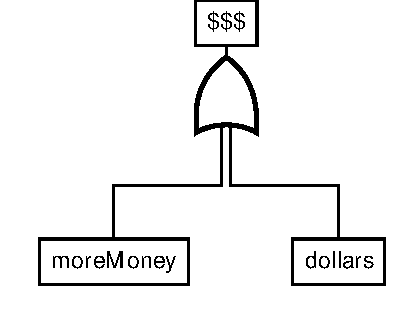
\includegraphics[ width=\textwidth]{graphviz/electrical_vs_consumer.pdf}
  \end{center}
  \vfill
  \begin{center}
    {\large
      Project Report%Insert document type (e.g., Project Report)
    }\\
    \vspace{0.2cm}
    {\Large
      DES904E15%Insert your group name or real names here
    }
  \end{center}
  \begin{center}
  Aalborg University\\
  Department of Computer Science
  \end{center}
\end{titlepage}
\clearpage

\thispagestyle{empty}
{\small
\strut\vfill % push the content to the bottom of the page
\noindent Copyright \copyright{} Aalborg University 2015\par
\vspace{0.2cm}
\noindent Here you can write something about which tools and software you have used for typesetting the document, running simulations and creating figures. If you do not know what to write, either leave this page blank or have a look at the colophon in some of your books.
}
\clearpage


\pdfbookmark[0]{English title page}{label:titlepage_en}
\aautitlepage{%
  \englishprojectinfo{
    Smart Meter Security %title
  }{%
    Distributed and Embedded Systems\\
    Prespecialization %theme
  }{%
    Fall Semester 2015 %project period
  }{%
    DES904E15 % project group
  }{%
    %list of group members
    Bruno Thalmann\\ 
    Mikael Elkiær Christensen\\
    Mikkel Sandø Larsen\\
    Stefan Marstrand Getreuer Micheelsen
  }{%
    %list of supervisors
    René Rydhof Hansen\\
    Mads Chr. Olesen
  }{%
    7 % number of printed copies
  }{%
    \today % date of completion
  }%
}{%department and address
  \textbf{Department of Computer Science}\\
  Aalborg University\\
  \href{http://cs.aau.dk}{http://cs.aau.dk}
}{% the abstract
  Here is the abstract
}


\cleardoublepage
\pdfbookmark[0]{Contents}{label:contents}
\pagestyle{fancy} %enable headers and footers again
\tableofcontents

\clearpage
\listoftodos

\chapter*{Preface\markboth{Preface}{Preface}}\label{ch:preface}
\addcontentsline{toc}{chapter}{Preface}

This report has been prepared by 9th semester Software Engineering students at Aalborg University, during the fall-semester of 2015.
It is a pre-specialization project, which should serve as a the preliminary work for one or more master theses.
It is expected of the reader to have a background in IT/software, due to the technical content.

References and citations are done by the use of numeric notation, e.g. [1], which refers to the first item in the bibliography.

We would like to thank our supervisor René Rydhof Hansen and co-supervisor Mads Chr. Olesen for their excellent supervision throughout the project period.

\vspace{\baselineskip}\hfill Aalborg University, \today

\vfill\noindent
\begin{minipage}[b]{0.45\textwidth}
 \centering
 \rule{\textwidth}{0.5pt}\\
  Bruno Thalmann\\
 {\footnotesize <bthalm11@student.aau.dk>}
\end{minipage}
\hfill
\begin{minipage}[b]{0.45\textwidth}
 \centering
 \rule{\textwidth}{0.5pt}\\
  Mikael Elkiær Christensen\\
 {\footnotesize <michri11@student.aau.dk>}
\end{minipage}
\vspace{3\baselineskip}
\begin{center}
\begin{minipage}[b]{0.45\textwidth}
 \centering
 \rule{\textwidth}{0.5pt}
  Mikkel Sandø Larsen\\
 {\footnotesize <milars11@student.aau.dk>}
\end{minipage}
\hfill
\begin{minipage}[b]{0.45\textwidth}
 \centering
 \rule{\textwidth}{0.5pt}
  Stefan Marstrand Getreuer Micheelsen\\
 {\footnotesize <smiche11@student.aau.dk>}
\end{minipage}
\end{center}

\cleardoublepage
%mainmatter
\pagenumbering{arabic} %use arabic page numbering in the mainmatter
%!TEX root=../master.tex
In order for us to discuss potential problems with any smart meter systems, we first need some background knowledge.
In this chapter we will first of all very shortly present what the smart grid and smart meters are, along with a short outline of potential problems.
Two big issues, privacy and remote access-ability, will be further elaborated as these are two of the biggest issues with any smart meter system.
Finally, some assumptions will have to be made about any future implementations in order to more concretely discuss any security-related problems and/or solutions, which is done by presenting a ``Smart meter context model''.

\section{Smart Grid and Smart Meters}\label{smart_grid_smart_meter}
A smart grid is an electrical grid supported by a net, allowing two-way communication, whereas earlier it was only one-way.
This allows for much more dynamic power supply and consumption, as suppliers will know more about their consumers, and consumers will have more options in regards to their consumption.

The outline of a smart grid can be seen in \cref{fig:background:smartgrid}.
This consists of three main actors:

\begin{itemize}
	\item Power suppliers such as Windmills, solar panels, traditional power plants and external suppliers.
	\item A net supplier such as a Datahub \footnote{Danish term from \cite{LOV_nr_575_af_18-06-2012}} and smart meters.
	\item End consumers such as smart homes/buildings.
\end{itemize}

\begin{figure}[H]
	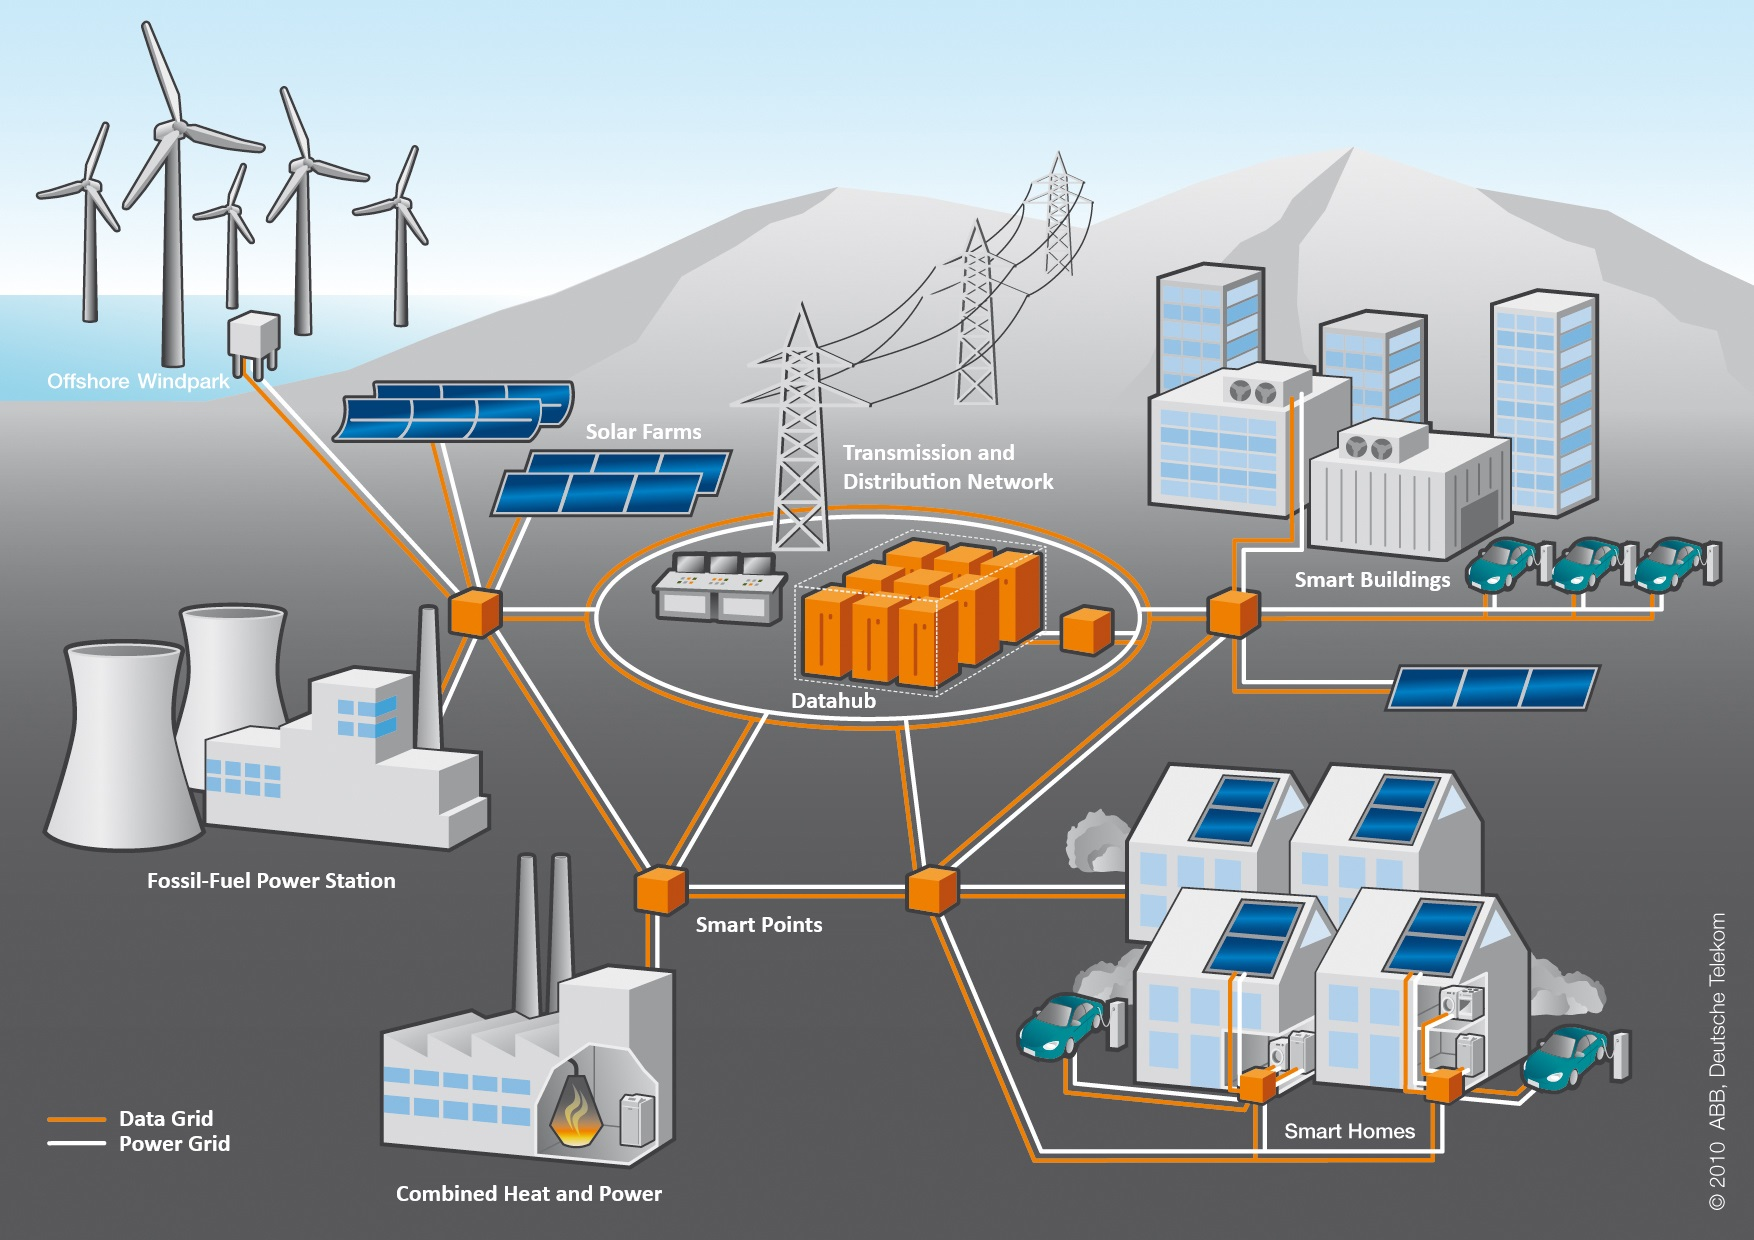
\includegraphics[width=\textwidth]{figures/SmartGrid_Ueberblick_ohneLegende.jpg}
	\caption{Smart grid outline\protect\footnotemark}
	\label{fig:background:smartgrid}
\end{figure}
\footnotetext{\url{https://www.telekom.com/medien/bild-ton-und-infografiken/infografiken/155030}}

A smart grid has several advantages over the old grids \cite{smartgrid_gov, directive_2009_72_EC}.
For instance it will enable prices to be base on supply and demand as well as the power source available.
Consumers will also be able to connect their own power generators such as windmills and solar panels.
Prices will then more realistically reflect environmental strain which can make the consumer more likely to consider the environment when consuming power.

The use of smart meters will also provide more detailed information about the power consumption of the consumer which enables the consumer to use smart appliances that can turn on when the power is cheap.
The consumer can also monitor the power usage and adjust his practices according to the prices.

On a large scale the smart grid also enables connecting the national grids across Europe for better utilization of the generated power.


\subsection{Smart appliances}
\label{background:smart_appliances}
Smart appliances\cite{smart_appliances} are ordinary appliances, such as air conditioners or dishwashers.
What makes them smart is the fact that the times or periods in which they are turned on are highly configurable, so that they can match changing power prices.
This can be done manually, by the user looking at current pricing and setting a timer when to turn on.
However, some smart appliances can also by themselves look up prices and choose appropriate times to turn on.

\subsection{Problems}
In regards to enabling an EU-wide smart grid, there are bound to be problems, as this is an immense project.
The roll-out will not be the same in every nation, as each nation has its own infrastructure and legal constraints.
Additionally they differ in which parts of their electrical grids are privately and publicly owned.
However, some shared problems still exist, such as privacy, conflicts of interest, and attack vulnerabilities \cite{offswitch, smart_meter_survey, security_economics}.

\subsubsection{Different architectures}
Even though the implementation of smart grid and smart meters is a EU project, they are not that specific when it comes to where responsibilities should lie.
It is up to each nation, depending on their current system and infrastructure, who should distribute smart meters and who will own the data.

Here are a few examples of different architectures \cite{smart_meter_survey}:
\begin{itemize}
	\item \textbf{Italy} - Regulated monopoly (supplier and distributor is the same).
	\item \textbf{Germany} - Free market for both distributor and supplier, households will have free choice in both.
	\item \textbf{UK} - Centralized government-licensed monopoly, which will have a datahub from which data will be distributed to suppliers, customers, etc.
	\item \textbf{Denmark} - Centralized through 60 government-regulated distributors, a government-owned datahub contains all data \cite{dk_marked,LOV_nr_575_af_18-06-2012}.
\end{itemize}

\subsubsection{Privacy}
With the adaptation of smart meters it will be possible to collect power usage data more often.
This is possible as it can be done remotely, whereas earlier a display would have to be read on the physical electrical meter.
It also makes sense to have more readings, as tariffs will vary more \cite{directive_2009_72_EC, eu_smart_meter_pricing}, and therefore more measurements are needed to match prices during tariff-determined periods.

This possibility of finer granularity meter readings can be exploited in several ways and by different actors.
The supplier would like this information in order to better tailor prices for a certain customer, thus limiting competition as their competitors do not possess this information.
If the power usage data was obtained by an electronics vendor, they could use it to target certain advertisements, based on what devices they detect (or do not detect) through the power usage.
Anyone with malicious intent could use the power data to determine who, if anyone, is home (e.g. burglars).
Finally, the government could use this data to surveil the public.

Some important issues with smart meters and their measurements are therefore:
\begin{itemize}
	\item Who owns the data?
	\item Who should be able to access the data?
	\item With which granularity should supplier/government/user be able to access the data?
	\item How do we ensure that only the correct people have access to the smart meter and its data?
\end{itemize}

\subsubsection{Conflict of interest}
The various actors involved with smart grids have different interests and potential gains.
Governments generally want lower consumption for environmental reasons.
They especially want consumption down during peak hours, in order to avoid the usage of environmentally unfriendly energy sources.
Depending on tariffs, suppliers might also want power consumption down during peak hours if they cannot provide enough, from their perspective, cheap energy.
However, suppliers generally want high consumption, so that they can sell more power and thus make more money.
Consumers want to use power as needed, but at lower costs.

These interests exemplify considerations by actors in a smart grid system.
Naturally there could be more such as consumers and suppliers having environmental considerations or governments seeking to increase productivity on a national level with lower regards for the environment.

The above relations spark several conflicts of interest:
\begin{itemize}
	\item Should governments be able to control user power consumption? If so, how?\footnote{E.g. carbon rationing in the UK \cite{security_economics}}
	\item Should others than the user be able to turn off the power? (See \cref{off_switch}) If so,
	\begin{itemize}
		\item who should be able to use this?
		\item how should it work? (With abuse in mind.)
	\end{itemize}
\end{itemize}

\subsubsection{Vulnerabilities}
In the current system consumeres are already tampering  with their mechanical electrical meters.
Turning these mechanical meters into smart meters will possibly remove attacks, but will definitely open up for new attacks.
Switching to smart meters introduces a new branch of attacks; digital attacks.
These include attacks that are general to any publicly exposed unit, or any unit that sends data over public networks.


\chapter{Related Work}
\section{Smart meter privacy concerns}

%!TEX root=../master.tex

\section{Concerns regarding the remote access-ability of smart meters}\label{off_switch}
As the smart grid and smart meters are getting more common an important observation was made by \citet{offswitch}.
This observation is regarding the possibility of the electrical company to switch off the smart meter.
The purpose of a remote off-switch could be to switch of the electricity if a customer is not paying.
When having smart meters controlled one place this place could be a target by terrorists, other countries or by a group of activists. 
\stefan{\#43 add til aktører og lav træer}
\paragraph{Large scale consequences}
In a scenario where millions of smart meters are deployed and controlled from a central control unit without taking possible attacks against the off-switch into account could be very dangerous.
\citet{offswitch} states that this is happening in the United Kingdom.
This means that there probably are a lot of vulnerabilities in the setup.
If an attacker gets access to the central control unit he has the ability to compromise all the connected smart meters.
By also tampering the cryptography of the smart meters the attack could last for weeks for some consumers.
People would die from basic diseases as for instance hypothermia because of lack of electricity at hospitals.
The region it would effect would be in chaos.

\paragraph{Attackers}
Possible attackers for such an attack could be:
\begin{itemize}
\item Countries when there is international tension.
\item A terrorist organisation.
\item Environmental activists which are frustrated with governments not taken the environment seriously.
\item A criminal who switches off all or some smart meters from an electrical company and demands money for switching them on again.
\end{itemize}
\stefan{samme liste blev nævnt i starten, skal det eventuelt slettes det ene sted?}
\mikael{I think the list is good, as long as it doesn't mention the exact same as above. The other mention could probably be shortened or generalized.}


\chapter{Theory}
%!TEX root = ../master.tex
\section{Protection in Operating Systems}
As most protection systems have different approaches to how they manage rights and chains of trust they are hard to compare on equal terms.
Additionally, it is often not easy to express which rights are leaked under certain conditions, or to whom they are leaked.
Oftentimes such leaks are only described informally by examining key features of a given system.

The model described in \citet{HRU} from 1976 can be used to solve these problems.
By formally describing protection systems using a unified model, they can be compared in terms of the rights that they leak.
Using this approach two possible solutions (protection systems) to a problem can be compared on even terms.

In the following the model proposed by \citet{HRU} is presented.

\subsection{Aprotection system}
A protection system can be described in terms of a set of rights $R$ and a set of commands $C$.
Both these sets are finite and static for a given system.
Because of this, a system cannot dynamically add or remove rights or commands, under this model.
\footnote{It is possible to simulate adding/removing predefined rights and commands in a system.}

\begin{definition}
  A protection system is a finite set of rights $R$ and a finite set of commands $C$.
\end{definition}

The rights of a protection system have no inherent semantics except for those implied by their use in commands.
Commands are used to modify the configuration of a protection system.
A definition of such a configuration is given below.
Note that $R$ and $C$ are not part of the configuration of a system, reflecting the definition of a protection system.

\begin{definition}\label{protection:def:state}
The state, or configuration, of a protection system is a triple $Q = (S, O, P)$, where $S$ is the set of \subjects{} in the configuration, $O$ is the set of objects in the configuration (with $S \subseteq O$) and $P$ is an access matrix describing the rights each \ssubject{} has to each object.
Finally $P[s, o]$ represents the cell in $P$ containing the set of rights that the \ssubject{} $s$ has to the object $o$ (with $P[s, o] \subseteq R$).
If no such rights exists we have that $P[s,o] = \emptyset$.
\end{definition}

We can represent a configuration $Q$ by annotating the access matrix with the associated \subjects{} and objects.
\Cref{protection:matrixsmall} shows an example of this approach in which there is a row for each \ssubject{} and a column for each object.

\begin{figure}[h]
\centering
\begin{tabular}{l|c|c|c|}
\multicolumn{1}{c}{} & \multicolumn{1}{c}{Sam} & \multicolumn{1}{c}{Joe} & \multicolumn{1}{c}{Data} \\\cline{2-4}
Sam & $\emptyset$ & $\emptyset$ & $\{\textbf{own}, \textbf{read}, \textbf{write}\}$ \\\cline{2-4}
Joe & $\emptyset$ & $\emptyset$ & $\{\textbf{read}\}$ \\\cline{2-4}
\end{tabular}
\caption{A representation of a protection system configuration}
\label{protection:matrixsmall}
\end{figure}

Transitioning from one configuration is done using commands.
A command can, through a set of operations, modify each part of the configuration tuple.
A command is defined as below:

\begin{definition}
A command takes a simple form, allowing for a name (here represented as $\alpha$), a condition, and a list of sequentially executed operations.
Let $X_i$ be \subjects{} and objects such that $X_i \in O \supseteq S$ and specifically $X_{s_i} \in S$ and $X_{o_i} \in O$.
Then a command is defined as:
\begin{algorithm}[H]
  \DontPrintSemicolon
  \SetKwFunction{cmda}{$\alpha$}
  \SetKw{cmd}{command}
  \SetKwBlock{block}{}{end}
  \cmd \cmda{$X_1, X_2, \cdots, X_k$} \block{
    \If{$r_1 \in P[X_{s_1}, X_{o_1}] \wedge r_2 \in P[X_{s_2}, X_{o_2}] \wedge \dots r_m \in P[X_{s_m}, X_{o_m}]$}
    {$operation_1$\;$operation_2$\;\dots\;$operation_n$\;}
  }
\end{algorithm}
%The arguments for a command are \subjects{} and objects; $X_i \in O \supseteq S$, however the use of these within the command come with certain restrictions.
%These restrictions are a direct result of the definition of $P$ and are that $X_{s_i} \in S$ and $X_{o_i} \in O$.
\end{definition}

\subsubsection{Operations}
The model described by \citet{HRU} is set to be as simple as conceivably possible.
Because of this only the list of operations in \cref{protection:operations} are allowed in commands.
No general purpose computation is directly possible using the proposed model as it does not reflect the protection aspect of the commands semantics.

The semantics of the available operations are formally specified in \citet[p. 463]{HRU}.
The operations and their associated semantics are quite self explanatory, performing simple updates of the access matrix.
Because of this they are not included here.

\begin{figure}[H]
 \centering
 \[\arraycolsep=14pt%\def\arraystretch{2.2}
 \begin{array}{l|l}
  \textbf{enter } r \textbf{ into } P[X_s, X_o] & \textbf{delete } r \textbf{ from } P[X_s, X_o]\\
  \textbf{create \ssubject{} } X_s & \textbf{create object } X_o\\
  \textbf{destroy \ssubject{} } X_s & \textbf{destroy object } X_o
 \end{array}
 \]
 \caption{The six primitive operations described by \cite{HRU}}
 \label{protection:operations}
\end{figure}

The application of an operation is written as $Q \Rightarrow_{op} Q'$ and thus $Q \Rightarrow_{op^*} Q'$ represents a sequence of operations.
An operation is executed by applying its changes to an access matrix resulting in a new access matrix.
If, for instance, we apply the \textbf{enter \textit{write} into $P[Joe, Data]$} operation to the access matrix described in \cref{protection:matrixsmall} we would have a new configuration reflecting the entered right.
The result of that operation can be seen in \cref{protection:matrixwithwrite}.

\begin{figure}[H]
\centering
\begin{tabular}{l|c|c|c|}
\multicolumn{1}{c}{} & \multicolumn{1}{c}{Sam} & \multicolumn{1}{c}{Joe} & \multicolumn{1}{c}{Data} \\\cline{2-4}
Sam & $\emptyset$ & $\emptyset$ & $\{\textbf{own}, \textbf{read}, \textbf{write}\}$ \\\cline{2-4}
Joe & $\emptyset$ & $\emptyset$ & $\{\textbf{read}, {\color{blue}\textbf{write}}\}$ \\\cline{2-4}
\end{tabular}
\caption{The configuration from \cref{protection:matrixsmall} with an added write right}
\label{protection:matrixwithwrite}
\end{figure}

Executing a command is then a matter of applying all of its operations in sequence or doing nothing, depending on the result of the conditional expression associated with the command.
The invocation of a command (with a set of arguments) is described as $Q \vdash_{\alpha(x_1, x_2, \cdots, x_k)} Q'$ and implies the description given above.

Should we want to give \textit{Joe} write access (as above) we might do this through a command that will only allow the owner of the data to provide write access.
An example of such a command is presented in \cref{protection:conferexample}.
With such a command the \textit{write} right to an object can only be given to a \ssubject{} by the owner of the object.

\begin{algorithm}
  \DontPrintSemicolon
  \SetKwFunction{cmda}{$confer_{write}$}
  \SetKw{cmd}{command}
  \SetKw{enter}{enter}
  \SetKw{into}{into}
  \SetKwBlock{block}{}{end}
  \cmd \cmda{owner, user, content} \block{
    \If{$own \in P[owner, content]$}
    {\enter{$write$ \into{$P[user, content]$}}\;}
  }
  \caption{Conferring write rights to another \ssubject{} \cite{HRU}\label{protection:conferexample}}
\end{algorithm}

\subsection{Analysis of protection systems}
Given the formal definition of a protection system we are able to ask specific questions about a given protection system.
By defining a set of requirements we can ask the same questions about several protection systems in an attempt to determine which system meets most or all of these requirements.
These questions could be any of the below:
\begin{itemize}
\item Does the system leak the right $r$?
\item Does the system leak the right $r$ to the \ssubject{} $s$?
\item Does the system leak the right $r$ to anyone other than \ssubject{} $s_1$, $s_2$, or $s_3$?
\end{itemize}
It should be noted that all these questions are answered on the basis of an initial configuration $Q$.
In other words; we are not interested in whether or not a right is leaked from an unattainable configuration.
Additionally, we might be interested in determining if a right can be leaked given a specific configuration, effectively deciding what effects a specific right will introduce in the system.

It should be noted that a leak (given in the definition below) is not necessarily a negative.
Certain rights we will want the system to leak in a specific way.
We are both interested in ensuring that certain rights are not leaked and that certain other rights are.

\begin{definition}
A command $\alpha$ leaks the right $r$ from configuration $Q$ if, after running $\alpha$ on $Q$, $r$ is entered into a cell in the access matrix where it did not exist before running $\alpha$.
A protection system leaks the right $r$ given an initial configuration $Q$ if there exists a command in the system that leaks $r$ from $Q$, or there exists a configuration $Q'$ which is reachable from the initial configuration such that there exists a command in the system that leaks $r$ from $Q'$.
\end{definition}

\subsubsection{Determine if a System Leaks}
We can translate the latter two types of questions, presented above, into the first one.
Because of this it is sufficient to provide an algorithm that will answer this type of question.

\begin{definition}
  There exists no general purpose algorithm for determining if a protection system leaks a right $r$ from configuration $Q$. \Cite{HRU}
\end{definition}

This is the major result described by \citet{HRU}.
There does, however, exist how such an algorithm for a very simple class of protection systems called mono-operational (a system of commands with only a single operation each).
Thus an algorithm exists for very simple system and not for complex systems.

In order to answer questions about specific protection systems, such as those in this chapter, custom algorithms must be defined.
These algorithms must be built such that they can be applied to the protection systems being tested.
The article does however not describe how to built such an algorithm.

%!TEX root=../master.tex

\newcommand{\policy}[2]{\ensuremath{#1\!:\;#2}}

\section{Decentralized Label Model}
The Decentralized Label Model (DLM) is an information flow control model.\cite{myers1999mostly}
As the name suggests it revolves around labels (similar to previous security models), however, DLM is decentralized.
This means that it can be applied to systems with no trusted third party, or even any trust throughout the system.
By attaching security labels to objects in code it can be controlled how information should be shared throughout the code and at code-endpoints (input/output to/from other programs).
It is possible to do both static and run-time checking of labels.
The final major point of DLM is that it is formalized and even though no implementation is supplied, it should be applicable to other existing programming languages.

\newcommand{\xvalue}{value}
\newcommand{\xvalues}{values}
This section describes DLM with small examples.

\subsection{Labels}
A \xvalue{} is associated with a label.
The label is a set of privacy policies.
When the \xvalue{} flows through the system, all the policies need to be obeyed.
This means that the effective set of \principals{} able to read the \xvalue{} is the intersection of all policies in a label.

A privacy policy is represented as an owner of some \xvalue{} and a set of readers.
The syntax is: $\policy{\text{<\emph{owner}>}}{\text{<\emph{reader}>}}$.
The owner is the \principal{} who owns the \xvalue{} that was used for constructing the \xvalue{}.
The readers are the \principals{} allowed by the owner.
The owner is implicitly allowed to read his own data.
If we want a \principal{} $p$ that should not allow any other readers we use the following syntax: $\policy{p}{}$.

If we have policy $K$ and label $L$, we have following notation:
\begin{itemize}
\item $K \in L$, policy $K$ is a part of label $L$
\item $\textbf{o}(K)$, the owner of policy $K$
\item $\textbf{r}(K)$, the set of readers of policy $K$
\end{itemize}

Labeled \xvalues{} are only released by the consensus of all the owners and can only be read by the readers.
If one or several privacy policies are added to a label it restricts the access to the \xvalue{}.
A label with no policies  means that all readers are allowed.

If a \principal{} is not among the owners of a label, it is the same as if it was added as a privacy policy with all posible readers, implicitly indicating that this owner has no preference of who reads the \xvalue{}.

\begin{example}{Redundant owner}
In a system with owners $o_1, o_2, o_3$ and readers $r_1, r_2, r_3$, the following labels are defined:
$$L_1 = \{\policy{o_1}{r_1,r_2};\; \policy{o_2}{r_2, r_3}\}$$
$$L_2 = \{\policy{o_1}{r_1,r_2};\; \policy{o_2}{r_2, r_3};\; \policy{o_3}{r_1, r_2, r_3}\}$$
Since the policy of $o_3$ is to allow everyone to read it introduces no restriction to the label.
Therefore we say that the effective reader set of the two labels are equal.
\end{example}

A label can contain several privacy policies for the same \principal{}.
These are enforced just as other policies.

\subsection{Rules}
This section contains the rules that need to be followed when manipulating labels to avoid information leakage.

\paragraph{Label join}
When deriving a \xvalue{} from two \xvalues{}, the derived \xvalue{}s' label must reflect its sources, so it has to be at least as restrictive.
The relation $\sqsubseteq$ determines that a label is \textit{at least as restrictive}.
\begin{definition}
  For two labels $L_1$ and $L_2$, if we have $L_1 \sqsubseteq L_2$, $L_1$ is at least as restrictive as $L_2$.
  Then, in order to keep the restrictiveness of a combination of two labels, the resulting label for a derived \xvalue{} is the union of the two source labels.
  This gives us the following join rule:
  \begin{center}
    $L_1 \sqcup L_2 = L_1 \cup L_2$
  \end{center}
\end{definition}

The join rule will ensure that any joining of values will also result in a joining of labels, so that any combination of rules will be upheld.

\paragraph{Relabeling by declassification}
The owners of the labels control their data, but sometimes policies are overly restrictive and one wants to relax them.
This can be used to sanitize \xvalues{} whose security policies, in respect to one ore more owners, have changed throughout the run of a program.
This works in opposition to restricting rules, which is used to ensure information is not leaked, whereas this is enabling intended leaking (of sanitized information).

The authority is a set of \principals{} which is the authority of the process of declassification.
If a process has the authority of a \principal{}, the actions of the process are permitted.
This means that if a \principal{} is in the authority set this can be declassified.

\begin{definition}
  A label $L_1$ can be relabeled to $L_2$ if $L_1 \sqsubseteq L_2 \sqcup L_A$ where $L_A$ is the authority.
  The authority is a label $L_A$ of the form $\{p: \ \}$ for every \principal{} in the current authority.
  $L_1$ can be relabelled to $L_2$ if $L_1 \sqsubseteq L_2 \sqcup L_A$ is true.
  \begin{center}
    \[\frac{L_1 \sqsubseteq L_2 \sqcup L_A}{L_1 \text{ may be declassified to } L_2}\]    
  \end{center}
\end{definition}

\paragraph{Relabeling by Restriction}
When a \xvalue{} is read from a variable it has the same label as the variable.
When a \xvalue{} is stored in a variable the label of the \xvalue{} is forgotten.
For example when doing an assignment:
\begin{example}{Assignment}
  Given $a = 4$, and we want to assign the value of another variable, $b$, to $a$.
  First we read the \xvalue{} from $a$, this means the \xvalue{} of $a$, $4$, has the same label as $a$.
  Now we assign the copied \xvalue{}, $4$, to $b$, this means the \xvalue{} gets the label of the variable $b$, replacing its own label.
  This means that the label that the \xvalue{} got from $a$ is forgotten.
\end{example}
This example shows the process of what we call relabeling, and more specifically this kind of relabeling is called restriction.

To avoid leakage the label of the variable must be at least as restrictive.
For instance if we have two labels, $L_1$ and $L_2$, $L_1 \sqsubseteq L_2$ means that $L_2$ is more restricted than $L_1$.

\begin{definition}
  So a restriction is when the new label guarantees to enforce all of the policies from the old label.
  If we have policy $J$ in $L_1$ it is guranteed by another policy $K$ if they have the same owner and $r(K)$ is a subset of $r(J)$.
  \begin{center}
    \[\frac{\forall (J \ \in \ L_1) \exists (K \ \in \ L_2)(o(K) = o(J) \ \wedge \ r(K) \subseteq r(J))}{L_1 \sqsubseteq L_2}\]    
  \end{center}
\end{definition}

\subsection{Acts-for relation}
A \principal{} in DLM can represent a user in the system, a group of users or roles.
As labels on slots are immutable, in order to have more dynamic security policies we have that \principals{} are able to \textit{act for} other \principals{}.
This means that a given \principal{} in effect has every right that the \principal{} that it acts for has.

This is also called a \principal{} hierarchy.
Formally we use the $\succeq$-operator when representing acts for.\footnote{$\succeq$ is reflexive and transitive and not anti-symmetric.}
For instance $x \succeq y$ means $x$ acts for $y$.
A \principal{} hierarchy $P$ is a set of ordered pairs of \principals{}.
So if we have $P \vdash x \succeq y$ it means that $(x,y) \in P$.

Some examples:
\begin{example}{Acts-for relation}
  Given the acts-for relation and \principals{} $Amy$ and $Bob$, $Amy \succeq Bob$ means that Amy \textit{acts for} Bob.
  Any security policies that apply to Bob will in effect also apply to Amy.
\end{example}
\begin{example}{Acts-for relation groups}
  Groups or roles are no different than any other principal -- given a new \principal{} $Admin$ we can have that $Amy \succeq Admin$, signifying that Amy is an administrator and therefore can act for on behalf of the administrator group. 
\end{example}
\subsection{Channels}
The model contains two channels, an input and an output channel.
Information can be leaked through these channels, therefore they have a label associated to them.
When a \xvalue{} enters the system through an input channel, the \xvalue{} gets the label of the input channel.
If a \xvalue{} is written to an output channel it can only be done if the label of the output channel is at least as restrictive as the label of the \xvalue{}.

\subsection{Smart Meter System Example}
In order to give some idea about how the DLM could be used, we provide an example of a smart meter system while displaying the different principals (actors) and labelled objects.
This is similar to the provided motivating examples presented in \cite{myers1997decentralized}.
However, this is very abstract and it is unsure in what degree an actual implementation would like this example, as many uncertainties involving the system and responsibilities still reside.

\begin{figure}[h]
\centering
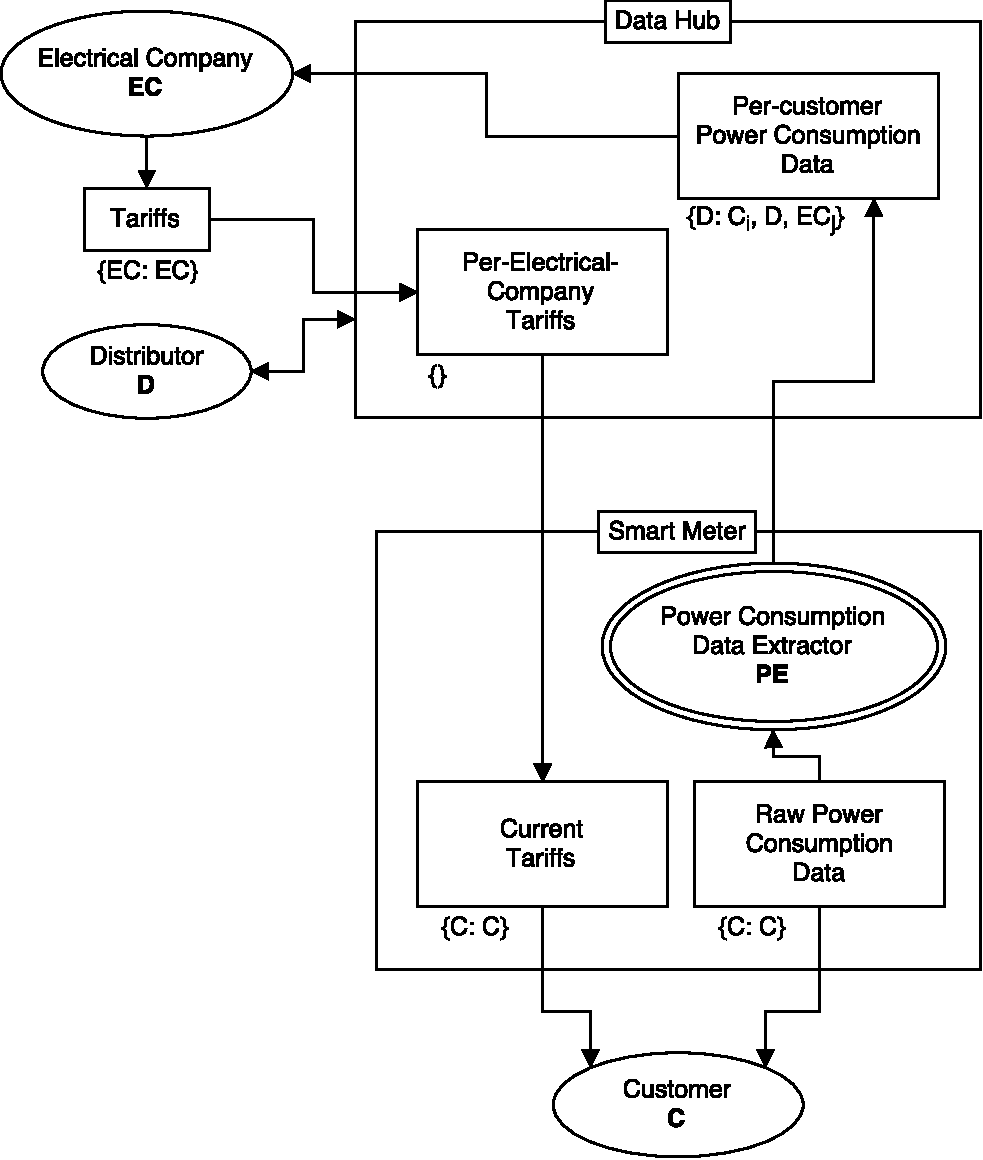
\includegraphics[width=\textwidth]{figures/dlm_sm_example.pdf}
\caption{Abstract smart meter system with DLM principals and labelled objects}
\label{dlm:sm_example}
\end{figure}

In \cref{dlm:sm_example} can be seen the abstract smart meter system, with principals (ovals), labelled objects (rectangles), and trusted agent (double oval).
Arrows display how information flows.
There are two overall components to this system: the Data Hub and the Smart Meter.
The rectangles used for these components signify only a grouping of objects.

Initially, consumers own the data contained in their smart meter, most importantly the raw consumption data.
In order for the distributor and electrical company to carry out their tasks, balancing the electrical grid and correctly billing, they have access to the transformed power consumption data.
Inside the data hub, the distributor receives ownership of all consumption data\footnote{This is actually unclear, but not important to discuss at this point}, but for the power consumption data for each individual customer $C_i$ the only allowed additional reader is the current electrical company of $C_i$: $EC_j$.
In case $C_i$ changes to a new electrical company $EC_k$, the read access must be removed from $EC_i$ and given to $EC_k$.

The different electrical companies will also provide their current tariffs to the data hub, so that they can be sent to the smart meters and for anyone to see the pricing of available electrical companies in case they want to switch supplier.
The label is empty so that anyone can read the tariffs.

\section{The Chinese Wall Security Policy}

The first security models that emerged were mainly concerned with military, and were thus tailored to fit the needs of the military. 
In \cite{brewer1989chinese} a model that is relevant for commercial applications is presented.
This model fits the needs of corporate business services like an analyst that must uphold the confidentiality of his clients, meaning that he cannot advise a corporation if he has insider knowledge of a competitor.
The following description is based on \citet{brewer1989chinese}.

\subsection*{The Chinese Wall Model}
A Chinese wall is defined as the separation between what can be accessed and what cannot be accessed by a user of the system.
Information is stored in a hierarchy with three levels. 
This hierarchy is depicted on \cref{hierarchy}.

\begin{itemize}
	\item The lowest level contains individual items of information, stored in objects.
	\item The middle level contains company datasets that group all information that concern one company. 
	\item The highest level contains conflict of interest classes which group companies that are in competition.
\end{itemize}

\begin{figure}[h]
  \resizebox{\textwidth}{!}{
	\begin{tikzpicture}


\node[fill=black,regular polygon, regular polygon sides=3,inner sep=1.5pt] (v3) at (-2,0) {};
\node[fill=black,regular polygon, regular polygon sides=3,inner sep=1.5pt] (v2) at (-3,0) {};


\node[fill=black,regular polygon, regular polygon sides=3,inner sep=1.5pt] (v4) at (-1,0) {};

\draw (v2) -- (v3) -- (v4);
\node (v7) at (-2,1) {Statoil};
\draw (v2) -- (v3) -- (v4);

\node (v14) at (0,1) {};
\node (v13) at (2,1) {Shell};
\node[fill=black, , regular polygon sides=3,inner sep=1.5pt] (v10) at (2,0) {};
\node[fill=black,regular polygon, regular polygon sides=3,inner sep=1.5pt] (v9) at (1,0) {};



\node[fill=black,regular polygon, regular polygon sides=3,inner sep=1.5pt] (v11) at (3,0) {};
\draw  (v9) -- (v10) -- (v11) ;

\node (v15) at (0,2) {Oil Companies};
\draw  (v14) edge (v15);




\node (v30) at (4,2) {};
\node (v40)at (8,2) {Banks};
\node (v23) at (8,1) {};
\node (v22) at (6,1) {Danske Bank};
\node (v24) at (10,1) {Spar Nord};
\node[fill=black,regular polygon, regular polygon sides=3,inner sep=1.5pt] (v25) at (10,0) {};
\node[fill=black,regular polygon, regular polygon sides=3,inner sep=1.5pt] (v28) at (9,0) {};



\node[fill=black,regular polygon, regular polygon sides=3,inner sep=1.5pt] (v29) at (11,0) {};
\node[fill=black,regular polygon, regular polygon sides=3,inner sep=1.5pt] (v18) at (6,0) {};
\node[fill=black,regular polygon, regular polygon sides=3,inner sep=1.5pt] (v17) at (5,0) {};



\node[fill=black,regular polygon, regular polygon sides=3,inner sep=1.5pt] (v19) at (7,0) {};
\draw (v17) -- (v18) -- (v19);

\draw (v23) -- (v40) -- (v30) -- (v15);
\node (v31) at (4,3) {Objects};
\draw  (v30) edge (v31);


\node at (-5,3) {\parbox{5cm}{The set of all objects}};
\draw[dashed, gray] (-3.8, 3) -- (v31);
\node at (-5,2) {\parbox{5cm}{Conflict of interest classes}};
\draw[dashed, gray] (-2.8, 2) -- (v15);
\node at (-5,0) {\parbox{5cm}{Individual data objects}};
\draw[dashed, gray] (-4.1, 1) -- (v7);
\node at (-5,1) {\parbox{5cm}{Company datasets}};
\draw[dashed, gray] (-3.4, 0) -- (v2);
\draw  (v3) edge (v7);
\draw  (v13) edge (v10);
\draw  (v22) edge (v18);
\draw  (v25) edge (v24);
\draw  (v7) edge (v14);
\draw  (v13) edge (v14);
\draw  (v22) edge (v23);
\draw  (v24) edge (v23);
\draw (v28) -- (v25) -- (11,0);
\end{tikzpicture}}
	\caption{The hierarchy of the Chinese Wall model.}
	\label{hierarchy}
\end{figure}

\paragraph{Example} A conflict of interest class could be \emph{Oil companies} which contains \emph{Statoil} and \emph{Shell}. \emph{Statoil} contains objects of information that could compromise the company if \emph{Shell} would obtain the information.

\subsection{The Security Policy}
The concept of the Chinese wall security policy is that a \principal{} that has access to information about company A which resides in a conflict of interest class C cannot access information about company B if B is also in conflict of interest class C.

In \cref{conflict} two companies are in the same conflict of interest class and a subject will not be able to access both of them at the same time.
Initially the subject will be able to choose freely from the two possibilities, but after choosing one of the companies the other will be unaccessible.

\begin{figure}[h]
  \centering
\resizebox{0.3\textwidth}{!}{  
  \begin{tikzpicture}


\node (v3) at (-2,0) {};
\node (v2) at (-3,0) {};
\node (v1) at (-3,-1) {};
\node (v6) at (-2,-1) {};
\node (v4) at (-1,0) {};
\node (v5) at (-1,-1) {};
\draw (v1) -- (v2) -- (v3) -- (v4) -- (v5);
\node (v7) at (-2,1) {A};
\draw (v6) -- (v3) -- (v7);



\node (v14) at (0,1) {};
\node (v13) at (2,1) {B};
\node (v10) at (2,0) {};
\node (v9) at (1,0) {};
\node (v8) at (1,-1) {};

\node (v12) at (3,-1) {};
\node (v11) at (3,0) {};
\draw (v8) -- (v9) -- (v10) -- (v11) -- (v12);
\draw (2,-1) -- (v10) -- (v13) -- (v14) -- (v7);
\node (v15) at (0,2) {C};
\draw  (v14) edge (v15);
\end{tikzpicture}
  }
  \caption{Two companies in the same conflict of interest class}
  \label{conflict}
\end{figure}

In \cref{conflict2} two companies are added to the system which results in the creation of a new conflict of interest class.
A subject will be able to access one from each conflict of interest class.
After choosing a company in conflict of interest class C, the subject still has a free choice from the two companies in conflict of interest class D.

\begin{figure}[h]
  \centering
  \resizebox{0.8\textwidth}{!}{
    \begin{tikzpicture}


\node (v3) at (-2,0) {};
\node (v2) at (-3,0) {};
\node (v1) at (-3,-1) {};
\node (v6) at (-2,-1) {};
\node (v4) at (-1,0) {};
\node (v5) at (-1,-1) {};
\draw (v1) -- (v2) -- (v3) -- (v4) -- (v5);
\node (v7) at (-2,1) {A};
\draw (v6) -- (v3) -- (v7);



\node (v14) at (0,1) {};
\node (v13) at (2,1) {B};
\node (v10) at (2,0) {};
\node (v9) at (1,0) {};
\node (v8) at (1,-1) {};

\node (v12) at (3,-1) {};
\node (v11) at (3,0) {};
\draw (v8) -- (v9) -- (v10) -- (v11) -- (v12);
\draw (2,-1) -- (v10) -- (v13) -- (v14) -- (v7);
\node (v15) at (0,2) {C};
\draw  (v14) edge (v15);




\node (v30) at (4,2) {};
\node (v40)at (8,2) {D};
\node (v23) at (8,1) {};
\node (v22) at (6,1) {K};
\node (v24) at (10,1) {J};
\node (v25) at (10,0) {};
\node (v28) at (9,0) {};
\node (v27) at (9,-1) {};
\node (v26) at (10,-1) {};
\node at (11,-1) {};
\node (v29) at (11,0) {};
\node (v18) at (6,0) {};
\node (v17) at (5,0) {};
\node (v16) at (5,-1) {};
\node (v21) at (6,-1) {};
\node (v20) at (7,-1) {};
\node (v19) at (7,0) {};
\draw (v16) -- (v17) -- (v18) -- (v19) -- (v20);
\draw (v21) -- (v18) -- (v22) -- (v23) -- (v24) -- (v25) -- (v26);
\draw (v27) -- (v28) -- (v25) -- (v29) -- (11,-1);
\draw (v23) -- (v40) -- (v30) -- (v15);
\node (v31) at (4,3) {O};
\draw  (v30) edge (v31);
\end{tikzpicture}
    }
  \caption{Introducing a conflict of interest class}
  \label{conflict2}
\end{figure}
This policy is being upheld by two properties, the \emph{simple security} property and the \emph{star property} corresponding to the identical properties defined in Bell Lapadula \stefan{ref til definitionen i Bellapadula}.

\paragraph{Simple Security}

When a \principal{} S requests to read an object O, this can only be permitted if one of the following requirements are fulfilled:

\begin{itemize}
\item O is in the same company dataset as an object already accessed by S (the object is within the wall)
\item O belongs to a entirely different interest class C than S has previously accessed
\end{itemize}

\paragraph{*-Property}

When a \principal{} S requests to write to an object O if the following requirements are both fulfilled.

\begin{itemize}
\item Access to O is permitted by the simple security rule
\item No objects from another object P in another company dataset D, which contains unsanitized information can be read when requesting write access to O
\end{itemize}

The second requirements ensures that unsanitized information cannot leave the company dataset, but it is still possible to sanitize the data in order to compare companies.

%!TEX root=..\master.tex
\section{Bell Lapadula}

Bell and LaPadula have devised a mathematical model intended for use in  military and governmental computer systems.
The model formalizes users accessing data and how to handle this in a secure way so confidential information cannot be leaked to a lower classification level.
The following description is based on \citet{lapadula1996secure}.

\subsection{Security}
Before we go into details about how the Bell-LaPadula (BLP) security model is applied to computer systems, we will first discuss some important concepts.

In any system we will have \textit{objects} and \textit{\subjects{}}, where objects are entities that can somehow be manipulated by the system's users (\subjects{}).
\Subjects{} can be users themselves, but can also be seen as representatives of a user or even groups of users.

\paragraph{Classification and Clearance}
Attached to any object or \subject{} will be a classification or clearance respectively.
This means that for any object $o$ with classification $x$, any \subject{} $s$ will need clearance $x$ or higher in order to access $o$.
In a hierarchical security system, where classification $y$ is a child of $x$, then an object given clearance $x$ will also have access to any objects with classification $y$.

\paragraph{Category and Need-to-know}
In addition to classification, objects can belong to zero, one or more category, which can be seen as security groupings of certain objects (e.g. ``Cold War'').
Similarly, \subjects{} can have zero, one or more need-to-know, which are the security groupings for \subjects{}.

\paragraph{Visualization}
This kind of security system can be seen as a \textit{lattice}, see \cref{blp:lattice}.
Each node represents an object, with a classification and possibly a category.
In the figure a \subject{} with the clearance \emph{Top secret} is able to read all nodes with the classification \emph{Top Secret} as well as all lower classifications (\emph{Secret} and \emph{Unclassified}).
On the contrary a \subject{} with the clearance \emph{Unclassified} can only read the one node with the \emph{Unclassified} label.

\begin{figure}
\centering
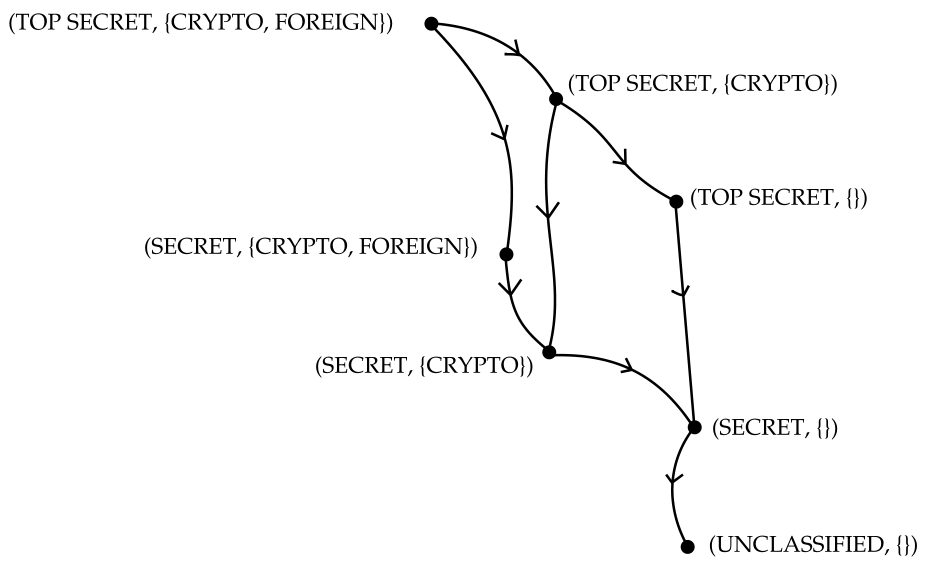
\includegraphics[width=\textwidth]{figures/blp_lattice}
\caption{A BLP lattice \cite{security_engineering_ross_anderson}}
\label{blp:lattice}
\end{figure}

\subsection{Access attributes}
The model considers four attributes for access in a complex computer system: \emph{read-only}, \emph{append}, \emph{execute} and \emph{read/write}.
In addition \emph{control access} is used to give attributes to other users.

\paragraph{Read-only}
This attribute makes it possible to read the object but not alter it.
The classical example is a file that contains information that should not be changed.
Alternatively it could be a list containing the \principals{} in the system with their clearance levels.
A \principal{} of low clearance should be able to read this list but not change it.

\paragraph{Append}
Append describes a pure write operation.
This means that it is possible to append information to the end of a file without being able to extract information about the rest of the file.

This can also be used with a printer which appends information about what is being printed.
By doing this it is sufficient that the classification of a piece of information is matching the classification of the printer in order to prevent unauthorized personnel from reading the information.

\paragraph{Execute}
The execution attribute makes it possible to execute an executable file.
If the \principal{} does not have permission to read from or write to the file he will only be able to execute it.
Similarly the executable file can produce output that is of a higher classification level than the clearance level of the \principal{} executing it.

\paragraph{Read/write}
This attribute signifies that read and write access are both allowed.
This attribute is what is traditionally used when editing text files.

\paragraph{Control access}
The control access attribute models the notion of a \principal{} having control over a file.
Having this attribute a \principal{} can give the four attributes above to other \principals{} in the system.

\subsection{Requests and decisions}
In a computer system the \principals{} are not directly accessing objects in the system, it is processes in the system that act on behalf of the \principal{}.
In the following a user requesting access to a file will be written as a \principal{} requesting access and the response to this request a decision
\stefan{to expand or not to expand? Det handler om hvordan hvordan de 5 access attributes skal handteres i en matrice. Er det nodvendigt for os?}
\bruno{Good question - would be nice to have as it is simplier to compare to the others that have access matrices - so depends on if we want that imo.}
\mikkelin{I am not sure that it is easier to compare, but I would like it because it adds something more concrete to the section.}
\mads{flueben}

\subsection{Preventing security compromise}\label{bellap:properties}
In order to ensure that data cannot be compromized the previous definitions of access attributes and requests can be utilized to formalize properties that ensure that compromise cannot occur.

\paragraph{Security condition}
The security condition states that a \principal{} with a given clearance level is prevented from having read access to any object which is or can be a source of information with a classification level that is higher than the clearance level of the \principal{}.

\paragraph{*-property}
The *-property states that if a \principal{} has write or append access to objects and read or read/write access to some objects, then the objects which he has write or append access to must exceed or equal the objects which he has read or write access to.
This property ensures that it is impossible to leak information to a lower classification level.

\mikkel{\issue{57} Gennemgående eksempel til BLP afsnittet}

In order to examine how a smart meter can be abused we need some basic security concepts.
In this chapter these concepts will be examined for later use.
First we will go over cryptography concepts and afterwards a selection of relevant attacks will be explained.

\section{Terms}
Alice and Bob are used to present two parties, this is so it is easier to understand.
Generally Alice wants to send Bob a secret message.
Eve is used as a third party which is eavesdropping on the communication between Alice and Bob.
This typical setup can be seen on \cref{alice_bob_eve}.

\begin{figure}[H]
  \begin{center}
    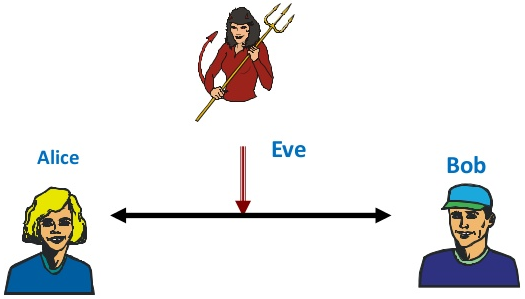
\includegraphics[width=.7\textwidth]{alice_bob_eve}
  \end{center}
  \caption[wat]{Alice, Bob and Eve.\footnotemark}
  \label{alice_bob_eve}
\end{figure}
\footnotetext{\url{https://image.slidesharecdn.com/quantumcryptography-130913005611-phpapp01/95/quantum-cryptography-13-638.jpg?cb=1379033822}}

%!TEX root = ../master.tex
\section{Cryptography}
This section will briefly introduce concepts from cryptography relevant to the project, and will be based on \cite{cryptoenginering}.

\subsection{Encryption}


\subsection{Authentication}
Authentication is a concept used for ensuring that the traffic between two parties are being tampered with.

When Alice sends messages to Bob over some insecure channel it can be possible for Eve to change how Bob receives the messages.
Eve can alter the sent message \emph{m} to \emph{m'} and send \emph{m'} to Bob without Bob knowing.
Eve can also change the order of messages so a message comes much later than intended.
If Eve deletes a message Bob will never know that this message existed.
Eve can even create her own message and send it without Bob can know that this message was not created by Alice.

\begin{figure}[H]
	\centering
	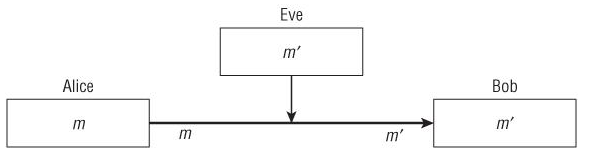
\includegraphics[width=0.6\textwidth]{authenticationNoAuth}
	\caption{The basic problem, who sent \emph{m'}? From \citet[p.~52]{cryptoenginering}}
	\label{crypto:noauth}
\end{figure}

Part of the solution to these problems is authentication of messages \citet[p.~52]{cryptoenginering}.
Alice and Bob have a shared secret key $K_a$ for authentication.
When sending message \emph{m} Alice first computes a Message Authentication Code (MAC).
This authentication code \emph{a} is calculated as $a := h(K_a,m)$, where $h()$ is the MAC function.
Alice now sends both the MAC \emph{a} and the message \emph{m} to Bob.
When Bob receives \emph{a} and \emph{m} he computes the MAC of \emph{m} and compares with the \emph{a} he received from Alice.
The situation is outlined on \cref{crypto:authsetup}

\begin{figure}[H]
	\centering
	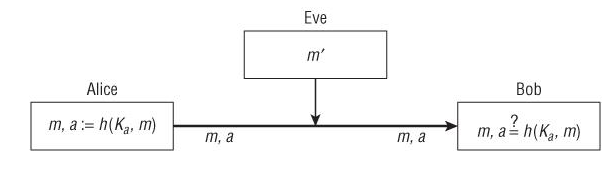
\includegraphics[width=0.6\textwidth]{authenticationSetup}
	\caption{Setup for authentication. From \citet[p.~53]{cryptoenginering}}
	\label{crypto:authsetup}
\end{figure}

If Eve wants to modify the message \emph{m} to the different message \emph{m'} and simply replaces \emph{m} with \emph{m'}, Bob will be able to tell when computing the MAC of \emph{m'}.
This is the case because of the design of the MAC function.
A MAC function is designed such that two different messages \emph{m} and \emph{m'} are very unlikely to result in the same MAC.
Bob will therefore discard message \emph{m} as an attacked message.

Even with this countermeasure Eve will be able to record a message and MAC pair and send it to Bob at a later point in time.
She can also still delete messages without Bob knowing that it ever existed.
Because of these flaws authentication is almost always accompanied by a numbering scheme which makes it possible for Bob to determine if there is being tampered with the message order.
Eve will still be able to entirely stop the communication between Alice and Bob, or delay it.

\stefan{noget om public key og digitale signaturer?}

%!TEX root = ../master.tex
\section{Network attacks}\label{attacks}

This section will contain attacks that work by interfering with network traffic.

\subsection{Replay attacks}\label{replay_attack}
This description of replay attacks is based on \citet[p.~223]{cryptoenginering}.

Eve can perform a replay attack if she is able to record a message from the communication between Alice and Bob.
She can then send the message to Bob at a later point in time. 

A related concept is retries.
During the run of a protocol Alice does not receive a response from Bob.
This could be because Bob did not receive Alice's request or a similar network problem.
To solve this Alice sends her message again.
This message is known as a retry.

Now Bob can receive both a replay from Eve and a retry from Alice.
Bob needs to deal with this properly so Eve cannot abuse replays to her advantage.
Abusing replays is known as a replay attack.

\subsection{Packet injection}
This description is inspired by \cite{packetinjection}.
If Eve can intercept communication between Alice and Bob she can inject packages into the stream of messages without either party knowing.
A packet is injected by constructing a packet with the source address as one of the endpoints, Alice or Bob.
In this way it looks like Alice or Bob originated the packet, and it seems like part of the communication.
By abusing this it can be possible to affect the communication of Alice and Bob.
Eve could be sending packets that simulate a protocol error, in order to disrupt the communication between Alice and Bob.
Or, by injecting new packets, Eve can alter the course of the communication, which can be dangerous if the communication involves sensitive information.

\section{Side channel attacks}
This description of side channel attacks is based on \citet[p.~132]{cryptoenginering}.

Side channel attacks is the class of attacks that take advantage of a alternate channels of information.
This could be how much time an operation takes, the power consumption during the operation or magnetic fields.

There are means for protecting against this type of attacks, but it is hard to eliminate information leakage from all possible channels.

\subsubsection{Differential Power Analysis}
One particular side channel attack is differential power analysis described in \citet{DPA}.
The article attacks a device encrypted with DES by recording power traces of the device performing encryption operations.
Because of the way semiconductors work, different operations will have a discernible signature on the power trace.
By recording enough traces information about the key can be derived from properties of the trace, and with enough traces the key can be derived.
\stefan{nok om DPA?}

\stefan{Hvis vi vil have mere om side channels: http://www.rambus.com/timing-attacks-on-implementations-of-diffie-hellman-rsa-dss-and-other-systems/}

\section{Buffer Overflow}
The following is based on \citet[p. 18]{foster2005buffer} and \citet[Section 1.1]{ruwase2004practical}.

A buffer overflow is an attack on a vulnerable program which modifies its memory state.
This gives the attacker the opportunity to control the machine where the program is executed with the same rights as the program(for instance ``root'').

A vulnerable program is a program that does not check if a given input exceeds its buffer size in memory.
If the program gets some input which exceeds its memory buffer size the program will copy the rest of the input in some adjacent buffer.


\section{Social engineering}
This section will contain attacks that abuses gullible individuals by psychologically manipulating them to performing some action.

\subsection{Phishing}

The following is based on \citet{security_engineering_ross_anderson} and \citet{dhamija2006phishing}.
Phishing is the process of tricking a user to give up sensitive information, such as user names or passwords, by posing as a trusted party.
This is typically done by using a malicious website, posing as a legit website that the user would normally use.
This could for example happen by inserting a fake link in an email and send it to the user.
The tricky part about phishing is to convince the user that the email with the link, and possibly the link itself, is legit.

An example could be a fake email to get a user's credentials for PayPal.
The email would contain the logo from PayPal and would tell the user to update his account information.
If the user then uses the link from the email he will get transferred to a malicious site.
When the user then enters his user name and password and submits it to the site the attackers will have his credentials.
To make it even worse for the user the attacker will redirect the user to real PayPal website and the user will have even less of a chance to know what happened.

\section{Malware}
The following is based on \citet[p.~644]{security_engineering_ross_anderson}.
Malware is collective name for malicious code. 
This includes \emph{trojans}, \emph{viruses}, \emph{worms} and \emph{rootkits}.
Common for these are that they infect a computer of a unsuspecting person and tries to achieve something harmful to either the person or his data.
For example a rootkit can provide control over the computer for the attacker while a virus can encrypt some crucial files on the hard drive and demand ransom.
A piece of malware could also install a backdoor in another piece of software, bypassing the intended security features.

In this context it is important to note that malware can provide access to a smart meter in a number of different ways.
If the password to the smart meter is stored on some client, malware will be able to send this back to the attacker.
A rootkit on a client will provide a possibility to control the smart meter through the client.



\chapter{Analysis}
\section{External Consumption Meter}\label{ecm}
An External Consumption Meter (ECM) is an electric meter which is attached to the incoming electricity phase(s) in the panel.
It consists of a measuring unit and a device to distribute these measurements, called an energy monitor.
The measuring unit is attached to the phase(s) and outputs raw measuring to the energy monitor.

The energy monitor can analyse the data and distribute them, this depends on which solution one chooses.
Some ECMs have an energy monitor which distributes the consumption data outside the home network and some also have the ability to analyse the consumption data.\cite{TED,efergy,open_energy_monitor}

Installing an ECM can be considered an attack because it can gather data about a person which can then be analyzed.
The implications of data gathered by an ECM were discussed in \cref{smart_meter_privacy}.

%!TEX root = ../master.tex
\section{Smart meter context model}\label{sec:smartmetercontext}

\begin{figure}[h]
  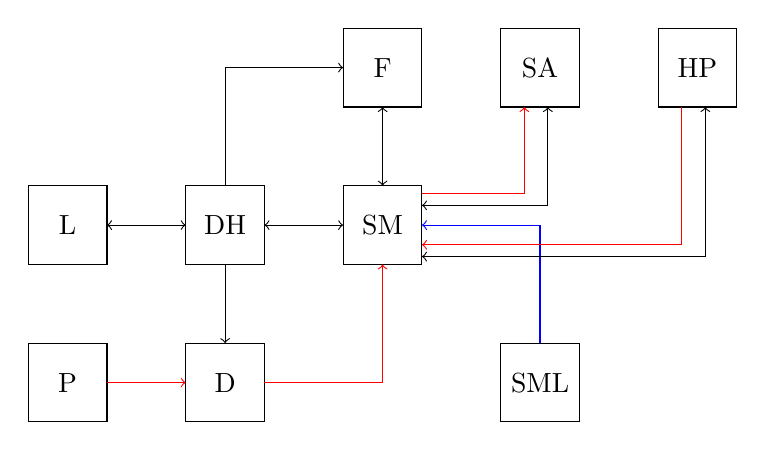
\begin{tikzpicture}
\newcommand*{\nodesize}{3}%

%\draw[help lines] (0,0) grid (10,10);


\draw (0,0) rectangle (1, 1) node[pos=.5] {P};
\draw[red, ->] (1, .5) -- (2, .5);
\draw (2,0) rectangle (3, 1) node[pos=.5] {D};

\draw (0,2) rectangle (1,3) node[pos=.5] {L};
\draw[<->] (1, 2.5) -- (2, 2.5);
\draw (2,2) rectangle (3,3) node[pos=.5] {DH};

\draw[->] (2.5, 2) -- (2.5, 1);

\draw (4,2) rectangle (5,3) node[pos=.5] {SM};

\draw[<->] (3,2.5) -- (4, 2.5);

\draw[red] (3,.5) -- (4.5,.5);
\draw[red, ->] (4.5, .5) -- (4.5, 2);

\draw (2.5,3) -- (2.5,4.5);
\draw[->] (2.5, 4.5) -- (4, 4.5);

\draw (4,4) rectangle (5,5) node[pos=.5] {F};

\draw[<->] (4.5, 3) -- (4.5, 4);

\draw (6,0) rectangle (7,1) node[pos=.5] {SML};

\draw[blue] (6.5,1) -- (6.5,2.5);
\draw[blue, ->] (6.5,2.5) -- (5,2.5);

\draw (6,4) rectangle (7,5) node[pos=.5] {SA};
\draw[red, <-] (6.3, 4) -- (6.3, 2.9);
\draw[red] (6.3,2.9) -- (5,2.9);

\draw[<-] (6.6, 4) -- (6.6, 2.75);
\draw[->] (6.6,2.75) -- (5,2.75);

\draw (8,4) rectangle (9,5) node[pos=.5] {HP};
\draw[red] (8.3, 4) -- (8.3, 2.25);
\draw[red, ->] (8.3, 2.25) -- (5,2.25);

\draw[<-] (8.6, 4) -- (8.6, 2.1);
\draw[->] (8.6,2.1) -- (5, 2.1);

\end{tikzpicture}
  \caption{The smart meter system\cite{tdlm}}
  \label{contextual:system}
\end{figure}

As no fully implemented smart meter systems currently exist, a lot of assumptions will have to be made before it is possible to imagine how such a system could be attacked.
We do this in two steps.

The first step taken is to outline the system as closely as possible.
Since there is no single correct system architecture, we have chosen the one opted by our native country: Denmark.
This system outline is based on the sources and information gained in the previous sections.

\subsection{The Smart Meter System}
The system is pictured in \cref{contextual:system}.
The lines indicate information flow between actors in the system.
The consumer (\textit{Household Owner/Residents}) can interact with the smart meter in order to control smart appliances and monitor the production of his home production devices.
\stefan{Vi mangler klient devices i vores model}
The \textit{Data Hub} stores the consumption data of the consumer.
This data is available for the consumer, the \textit{Distribution Companies} and the \textit{Electrical Company}.
These three actors have permission to see the consumption data in different granularities.
The consumer can see the data in the finest granularity, whereas the distribution companies and the electrical companies has access to a coarser granularity that makes it possible for them to calculate the bill.

\textbf{Note:} The electrical companies send price information to the data hub (not pictured), which the consumer can see through the smart meter.
\stefan{skulle vi overveje at inkludere det på billedet? \#99}

\subsection{Actors and threats}
Placing a smart meter in a consumers home and simultaneously requiring external access to its data is a complicated task with many potential risks.
\Cref{contextual:sm_model} represents this context and the actors therein.
This has been used as a starting point for a brainstorm that maps the potential attacks on the system.

\begin{figure}[h]
  \centering
  \tikzstyle{man}=[font={\Gentsroom}, scale=5]
\tikzstyle{woman}=[font={\Ladiesroom}, scale=5]

\begin{tikzpicture}[every node/.style={inner sep=0,outer sep=0}, arrows={[round]}]

\draw (-5.5,6) rectangle (2,-0.5);
\node at (-1,5.5) {Household};

\draw  (-6.5,7) [fill=white] rectangle (-4,5.5) node[pos=.5,align=center] {Home\\Production};
\draw  (-5,1.5) [fill=white] rectangle (-3.5,0) node[pos=.5,align=center] {Smart\\Meter};
\draw  (-3,4.5) [fill=white] rectangle (-1,3) node[pos=.5,align=center] {Smart\\Appliance};
\draw  (-0.5,2) [fill=white] rectangle (0.5,1) node[pos=.5,align=center] {Client};
\draw  (-9,2.5) [fill=white] rectangle (-6.5,1) node[pos=.5,align=center] {Data Hub};

\node[man] (consumer) at (1,1) {};
\node [below=0.2 of consumer] {Consumer};

\node[man] (burglar) at (-6.5,0) {};
\node [below=0.2 of burglar] {Burglar};

\node[man] (external) at (3.5,5) {};
\node [below=0.2 of external] {External};

\node[man] (power) at (-7.5,6.5) {};
\node [below=0.2 of power,align=center] {Electrical\\Company};

\node[man] (distribution) at (-7.5,4) {};
\node [below=0.2 of distribution] {Distribution};

\node[woman] (partner) at (1,4) {};
\node [below=0.2 of partner] {Partner};

\node[man] (neighbour) at (3.5,0.5) {};
\node [below=0.2 of neighbour] {Neighbour};

\draw[dashed] (-4.5,5.5) -- (-4.5,1.5);
\draw[dashed] (-6.5,1.5) -- (-6,1.5) -- (-6,1) -- (-5,1);
\draw[dashed] (-3.5,1) -- (-2.5,1) -- (-2.5,1.5) -- (-0.5,1.5);
\draw[dashed] (-2.5,3) -- (-2.5,2.25) -- (-4,2.25) -- (-4,1.5);

\end{tikzpicture}
  \caption{The smart meter context model}
  \label{contextual:sm_model}
\end{figure}

\paragraph{Actors}\label{contextActors}
Below is the list of the actors represented in the full system and context.
The list below will briefly describe the actors, their objective, and how they can abuse a smart meter to achieve their objective.
\begin{itemize}
\item \textbf{Consumer}\\
The resident of the depicted home and the one whose power consumption is monitored.
The smart meter is installed in the consumer's home.
The consumer may want to attack his own smart meter in order to reduce his power bill.
\item \textbf{Burglar}\\ A burglar can use the smart meter to find out when the consumer is home, in order to break in, as well as finding out which products the consumer owns, in order to assess him as a target.
\item \textbf{Neighbour}\\
The next door neighbour to the consumer.
We assume that the neighbour will perform attacks on the consumer in order to remove annoyances, such as loud appliances or music.
In case of neighbourly disputes, messing with the SM and connected appliances could also be viable strikes.
\item \textbf{Partner}\\
The consumer's partner.
In this context there is no distinction between a partner who is living with the consumer and one that is not.
The partner would like to surveil or get revenge over the consumer, in case of misdoings on the consumer's part -- such as adultery.

\item \textbf{Electrical Company}\\
The company billing the consumer for his power consumption.
The electrical company may want to increase the bill of the consumer.
\item \textbf{Distribution Company}\\
Manages the part of the grid closest to the consumer and provides him with electricity.
Installs the smart meters in the consumer's home.
Government-controlled intermediary between the electrical company and the consumer.
The distribution company therefore has no gain from abusing the smart meter.
\item \textbf{External}
\begin{itemize}
\item \textbf{Information gatherers}\\ 
Some companies depend on information about consumers and can use the information provided by the smart meter to profile consumers.
\item \textbf{Developers of third party apps}\\
The developer of apps that the consumer will use for monitoring his electrical consumption. 
These apps can be either mobile, desktop, and web applications.
The information gatherer can abuse this position in order to collect data about the consumer and possibly sell it.
\item \textbf{Appliance company}\\ The provider of home appliances that can connect with the smart meter.
Can collect data through appliances and possibly sell it.
\item \textbf{Government}\\
The government officials (including counties and municipalities).
\item \textbf{States}\\ In countries with tension between them, one country could have an interest in abusing smart meters to attack citizens of the opposing country.
\item \textbf{Terrorist organisations}\\ Terrorists can abuse the smart meter for terrorist acts, like shutting off power in a city or region.
\item \textbf{Environmental activists}\\ Activists can abuse the smart meter as a means of demonstrating environmental politics.
\item \textbf{Blackmailer}\\ A criminal who switches off all, or some, smart meters from an electrical company and demands money for switching them on again.
\end{itemize}
\end{itemize}

\paragraph{Objects}
\begin{itemize}
\item \textbf{Smart Meter}\\ Controls and records power consumption for home appliances.
\item \textbf{Smart Appliance}\\ Optionally controlled from the smart meter.
For instance a washing machine can be started and stopped when scheduled.
\item \textbf{Data Hub}\\ Consumption data is stored on the Data Hub, which makes it available for the distributor and the electrical company.
\item \textbf{Home Production}\\ The consumer can connect his own home production devices such as solar cells or windmills.
\end{itemize}

\subsubsection{Smart Meter}
The following describes the conceptual smart meter we have used in our considerations, based on \cref{smart_grid_smart_meter}, \citet{tdlm}, and \citet{smart_meter_survey}.
These assumptions will be used throughout the report.
\begin{itemize}
	\item The smart meter is installed in the household of the consumer, in this case a house.
	\item Home appliances are connected to the smart meter and can be managed from it.
	\item The smart meter can be accessed through an API.
	\item The consumer can access and manage his home appliances connected to the smart meter through some sort of program, e.g. an app developed by a third party.
	\item The smart meter manufacturer has the ability to update software. \stefan{det har vi vel slet ikke brugt?}
	\item The home appliance company can update the firmware of their appliances through the smart meter.
	\item The smart meter sends its consumption data to the Data Hub.
	\item The electrical company have the ability to switch off the smart meter 
	\item The electical company obtains billing information from the Data Hub.
	\item Home production of electricity, for instance a windmill, is also connected to the smart meter.
\end{itemize}


\newcommand{\noattack}{N/A}
\newenvironment{attacktable}[2]
{
  \begin{tabular}{|p{2.2cm}*{#1}{|p{#2}}|}\hline
 & \multicolumn{#1}{|c|}{Attacks made against} \\ \hline
}
{
  \\\hline
  \end{tabular}
}
\newenvironment{attacklist}
{
  \begin{itemize}
  \setlength{\itemsep}{0em}
  \setlength{\parskip}{0pt}
  \setlength{\parsep}{0pt}
}
{
  \end{itemize}
}
\newcommand{\header}[1]{\multicolumn{1}{|c|}{#1}}

\begin{attacktable}{1}{10cm}
& \header{Distributor} \\ \hline
Consumer &
\begin{attacklist}
\item Report a lower consumption.
\item Upload own firmware / login as distributor.
\item Crack SM open and connect external hardware.
\item Intercept packages and falsify them.
\item Side channels (intercept keys)
\end{attacklist}
\end{attacktable}

\begin{attacktable}{2}{5cm}
& \header{Consumer} & \header{Appliance} \\ \hline
Distributor
&
\begin{attacklist}
\item Manipulate the measured data stored by the SM in a way that the user cannot detect. A marginal change in the data can be marginal as to not arouse suspicion.
\begin{attacklist}
\item Change in the way data is stored.
\item Change in the stored data.
\end{attacklist}
\item Bill the user incorrectly.
\item Extract and sell information about the type of appliances the consumer has.
\item Turn on appliances when favorable to the distributor.
\end{attacklist}
&
\begin{attacklist}
\item Preference to specific products in return for payment.
\end{attacklist}
\end{attacktable}

\begin{attacktable}{2}{5cm}
& \header{Consumer} & \header{Appliance} \\ \hline
Developers of\newline 3rd party apps
&
\begin{attacklist}
\item Develop app that looks \textit{right}, but uploads private information to the developer.
\item Develop app that looks \textit{right}, but reports incorrect consumption.
\begin{attacklist}
\item E.g. An electrical company that reports incorrect values when the user uses a different electrical company.
\end{attacklist}
\item Turn off appliances (trolling)
\end{attacklist}
&
\begin{attacklist}
\item Incorrect information about usage that favors specific appliances or specific appliance producers.
\item Have specific appliances appear to be defect.
\end{attacklist}
\end{attacktable}

\begin{attacktable}{1}{10cm}
& \header{Consumer} \\ \hline
Neighbors
&
\begin{attacklist}
\item Turn off appliances because they are noisy.
\item Connect appliances to the neighbors SM.
\end{attacklist}
\end{attacktable}

\begin{attacktable}{1}{10cm}
& \header{Consumer} \\ \hline
Burglar
&
\begin{attacklist}
\item Check to see if the consumer is at home.
\item Attempt to determine how many (and which) appliances the consumer has.
\end{attacklist}
\end{attacktable}

\begin{attacktable}{1}{10cm}
& \header{Consumer} \\ \hline
Girlfriend
&
\begin{attacklist}
\item Check if there is anyone at home.
\item Check which appliances are on.
\item Erase consumer as user from the SM.
\item Turn off the consumers appliances.
\end{attacklist}
\end{attacktable}

\begin{attacktable}{3}{3.3cm}
& \header{Consumer} & \header{Distribution} & \header{Appliance company} \\ \hline
Appliance \newline company
&
\begin{attacklist}
\item Appliances sending information about usage to the producer of the appliances.
\item Have SM display a lower consumption for an appliance than the actual consumption.
\end{attacklist}
&
\begin{attacklist}
\item Have SM display a lower consumption for an appliance than the actual consumption.
\end{attacklist}
&
\begin{attacklist}
\item Have SM display a lower consumption for an appliance than the actual consumption, such that it will look better when compared to competitors.
\end{attacklist}
\end{attacktable}
\bruno{Brug den her til inspiration til: \# 18}

%!TEX root=../master.tex

\section{Attack Trees}
Based on the model of the system describing the relations between actors and devices, a brainstorming session in the project group has led to a set of possible attacks on the system.
In the figure below (\cref{contextual:sm_model_attack}), which is an update of \cref{contextual:sm_model}, the result of this brainstorming session is visualized.
An arrow pointing from actor $A$ to actor $B$ indicates a possible attack by $A$ on $B$.

\begin{figure}[H]
  \centering
  \tikzstyle{man}=[font={\Gentsroom}, scale=5]
\tikzstyle{woman}=[font={\Ladiesroom}, scale=5]

\begin{tikzpicture}[every node/.style={inner sep=0,outer sep=0}, arrows={[round]}]

\draw (-5.5,6) rectangle (2,-0.5);
\node at (-1,5.5) {Household};

\draw  (-6.5,7) [fill=white] rectangle (-4,5.5) node[pos=.5,align=center] {Home\\Production};
\draw  (-5,1.5) [fill=white] rectangle (-3.5,0) node[pos=.5,align=center] {Smart\\Meter};
\draw  (-3,4.5) [fill=white] rectangle (-1,3) node[pos=.5,align=center] {Smart\\Appliance};
\draw  (-0.5,2) [fill=white] rectangle (0.5,1) node[pos=.5,align=center] {Client};
\draw  (-9,2.5) [fill=white] rectangle (-6.5,1) node[pos=.5,align=center] {Data Hub};

\node[man] (consumer) at (1,1) {};
\node [below=0.2 of consumer] {Consumer};

\node[man] (burglar) at (-6.5,0) {};
\node [below=0.2 of burglar] {Burglar};

\node[man] (external) at (3.5,5) {};
\node [below=0.2 of external] {External};

\node[man] (power) at (-7.5,6.5) {};
\node [below=0.2 of power,align=center] {Electrical\\Company};

\node[man] (distribution) at (-7.5,4) {};
\node [below=0.2 of distribution] {Distribution};

\node[woman] (partner) at (1,4) {};
\node [below=0.2 of partner] {Partner};

\node[man] (neighbor) at (3.5,0.5) {};
\node [below=0.2 of neighbor] {Neighbor};

\draw[dashed] (-4.5,5.5) -- (-4.5,1.5);
\draw[dashed] (-6.5,1.5) -- (-6,1.5) -- (-6,1) -- (-5,1);
\draw[dashed] (-3.5,1) -- (-2.5,1) -- (-2.5,1.5) -- (-0.5,1.5);
\draw[dashed] (-2.5,3) -- (-2.5,2.25) -- (-4,2.25) -- (-4,1.5);

\draw[ultra thick, red, -{Stealth[scale=1.2]}] (neighbor) -- (consumer);
\draw[ultra thick, red, -{Stealth[scale=1.2]}] (partner) -- (consumer);
\draw[ultra thick, red, -{Stealth[scale=1.2]}] (burglar) -- (consumer);
\draw[ultra thick, red, -{Stealth[scale=1.2]}] (external) -- (consumer);
\draw[ultra thick, red, -{Stealth[scale=1.2]}, bend right=90] (power) to[out=-10,in=190] (consumer);
\draw[ultra thick, red, -{Stealth[scale=1.2]}, bend right] (consumer) to[out=-10,in=190] (power);

\end{tikzpicture}
  \caption{The routes of attacks in the context model}
  \label{contextual:sm_model_attack}
\end{figure}

From this representation of the attacks it is evident that the consumer is threatened by the largest number of attackers.
Meanwhile he only has a single actor to perform an attack on.
This attack is described in \cref{attacks:consumer_vs_electrical}.

The consumer is not found to have an attack on the power distributor (or vice-versa) as the price of transporting electricity is governmentally regulated.
Additionally it is worth mentioning that there are no attacks that do not involve the consumer.

\paragraph{Definition of an attack tree}
Attack trees consist of a set of nodes representing steps in a possible attack.
The root node being the goal and leaf nodes being different ways to achieve this goal.
Inner nodes are represented as logic gates such that they do not represent a possible attack themselves but rather a rule describing how their children should be aggregated.
Thus a node represented by an AND gate would require all its child-nodes to be carried out successfully for it to be carried out successfully.

To describe an attack tree, for instance how feasible it is, nodes can have different values corresponding to different variables(Boolean and continuous).
For instance a variable could be \textit{cost} and the values assigned to it could be in dollars.
Attack trees can show you which attacks are possible for which attackers.
For instance an attacker with a lot of money has the possibility to do all the expensive attacks where a poor attacker has not.
Also if one builds a system where the data that is getting protected is not very important, it might only be important to defend against cheap attacks.
Making attack trees takes a lot of time and effort as one has to study the security measures in place, the possible attacks and the possible attackers and outline this information in one or more attack tree(s).\cite{schneier_attack_trees}

\section{Burglar}
This section will contain an analysis of the case that a burglar wants to break into the house of the consumer.
The attack tree presented in \cref{attacktree:burglar} contains both means that attempt to exploit the smart meter, as well as physical means.
Both alternatives are presented in order to be able to annotate the tree with weights to determine whether the smart meter attacks are actually valid as an entrypoint.

\begin{figure}
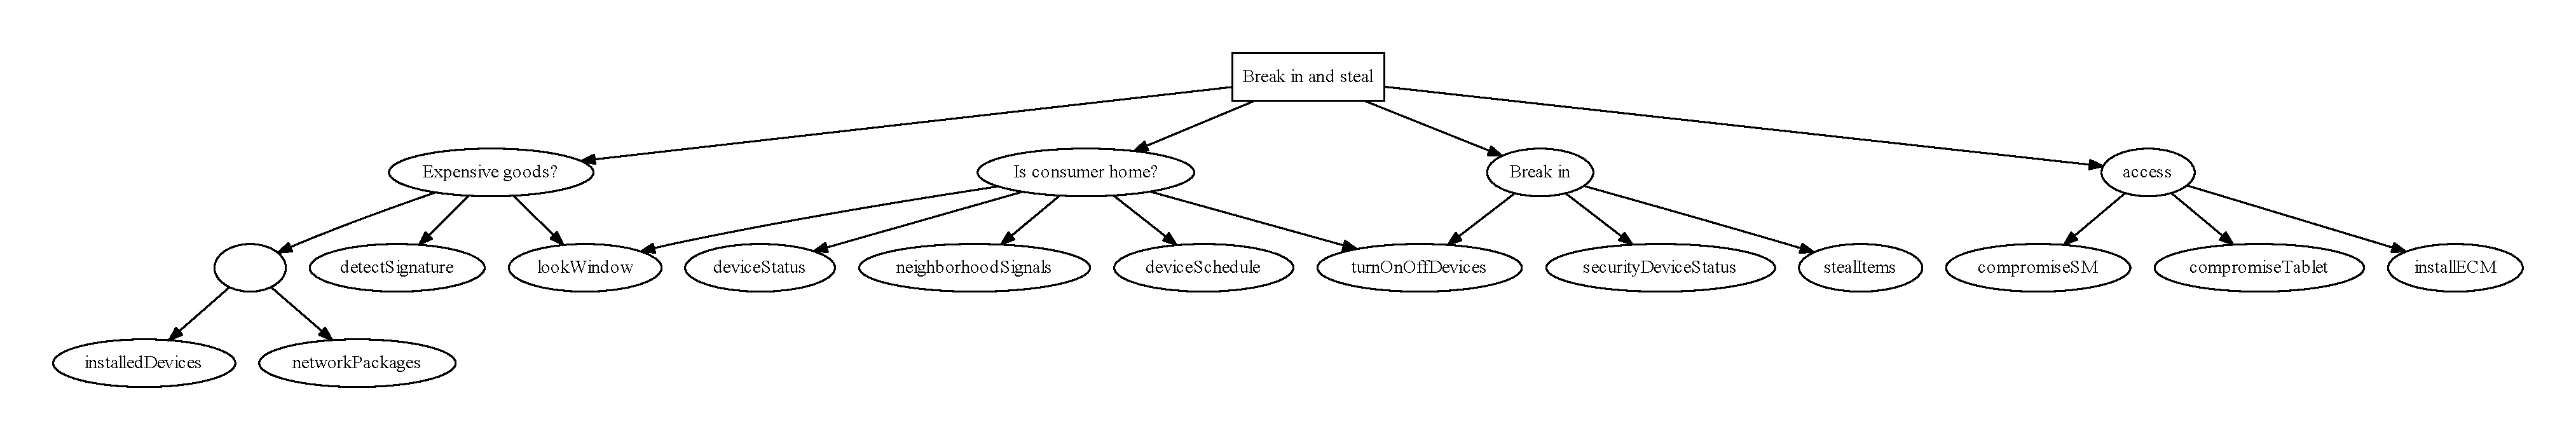
\includegraphics[width=\textheight, angle=90]{graphviz/burglar.pdf}
\caption{Attacktree of a burglar attacking the consumer}
\label{attacktree:burglar}
\end{figure}

\subsection{Tree}

\subsection{Gaining access}
In order to access any information of the power consumption of the consumer, the burglar needs to gain access to either the smart meter, the tablet that controls the smart meter or the power consumption through a different medium
\stefan{skal vi skrive en fælles del om dette?}

\subsection{Expensive goods}
The first step for the burglar is to determine if anything is of value in the house. 
The burglar can choose any house he wants, so he will probably assess which house will yield the highest total worth for the least effort.

The physical method is simply to look in through windows of the house and consider what can be seen. 
This method has some obvious shortcomings.
Not everything can be seen from the outside, and in multiple story houses several stories may be impossible to evaluate.
Is is also rather inaccurate - it may be possible to see a TV, but it is the newest product from this year, or is it an older model that is virtually impossible to sell?

If the burglar has compromised either the smart meter or the internet router of the consumer he will be able to find out what products are in the home. 
This is possible either through some smart meter database that shows what can be controlled, or through network traffic which can indicate what products are being communicated with.

If the burglar has access to the power consumption (either smart meter or the ECM), it will be possible to detect product signatures in this data.
This is difficult and possibly ambiguous, but it may provide pointers on what he can expect to find.
\stefan{evt. ref til memoir?}

\subsection{Is the consumer at home?}
When the burglar decides the home to be his target he needs to plan when to break in.
Before doing that he needs information about when the consumer is home.

Again he can use some physical methods to determine this.
He can look through the windows to check for activity in the house.
This technique is not guaranteed to show that he is not a home, but if there is activity the burglar can be sure that he is at home.
Over a longer period of time this technique can provide information about the habits and work hours of the consumer, making it easier to plan when to break in and when to be out again.

Another technique is to put indicators in the neighborhood.
This could be small signs on the mailbox, a can behind the wheel of a car or a knocked over bike.
The purpose of these subtle indicators is to find out if someone is not home for a longer period of time.
If the consumer is home he will with great probability stand up the bike or remove the mark from the mailbox.
But if he is not at home the burglar will be able to see this from the indicator.
This technique works particularly well if the burglar has several targets in the neighborhood, because he can just choose the house that has no activity.

If the burglar has access to the smart meter or an ECM he has some options that can help him determine if the consumer is at home.
From the power consumption is would be possible to determine what devices are currently on. 
If the TV is turned on and off in irregular intervals (timers exist that can turn devices on and off at predetermined intervals), it is an indicator that he is home.

Also schedule information can be an indicator if he is at home.
If the consumer schedules clothes washing during the night it must indicate that he plans to be home some time after the ended clothes wash.
The schedule may also provide information about work hours of the consumer making it possible for the burglar to plan the break in

Having control over the smart meter also provides the power to turn devices on or off.
The burglar can use this to reinforce any suspicion he has that the consumer is or is not home.
If he thinks that the TV is turned on by some timer mechanism he can force it to turn off.
If the consumer is really at home he will probably turn it on again.
Provided that this action must be done manually, this is an surefire proof that he is at home.
Another test could be to turn the stereo on and put the volume to an abnormally high level.
If the consumer does not react to this, he is either sleeping very tight or not at home.

\subsection{Break in}
When the burglar feels confident that he wants to break into the house he can use the smart meter for some additional help.
The smart meter can provide information about the security status of the house.
Is there is security alarm or security camera this will be visible on the smart meter by the same techniques mentioned in the "Expensive goods" subtree - either in the consumption data, network data or smart meter database.
If the consumer has some security devices installed he can turn them off entirely and make the break in easier without even entering the property.

The last step is to steal all the expensive goods in the house of the consumer.
The smart meter (as well as surveillance) can have provided information the tells the burglar when the consumer is usually home, and he therefore know when to be out in order to not get caught.
%!TEX root=../master.tex

\section{Partner attacking the Consumer}
The partner is an actor with relation to the consumer, but unlike the other actors partners usually can get away with more misdoings inside the consumer's property or house.

With this attack the partner wishes to monitor the consumer, possibly with following revenge, if monitoring leads to the conclusion that the consumer was cheating on the partner.
What distinguishes the partner's attacks from the burglar's and neighbour's is that the partner has increased access to the consumer's property, including the smart meter and related objects.

The attack trees are separated into the four modes of access for the same reasons as the burglar (see \cref{attacktree:burglar}) was.
The attack trees are listed below

These are listed below:
\begin{itemize}
  \item \Cref{fig:attack_trees:partner:cheater_sm}: Compromising the security on the smart meter.
  \item \Cref{fig:attack_trees:partner:cheater_client}: Compromising or extracting data from the device (the client) the consumer is using to communicate with the smart meter.
  \item \Cref{fig:attack_trees:partner:cheater_ecm}: Installing an ECM and monitoring the consumer.
  \item \Cref{fig:attack_trees:partner:cheater_physical}: Performing a \emph{``physical''} attack, involving no technology.
\end{itemize}

Each tree represents the possible attacks and gains, depending on the kind of access acquired.
There are two or three overall steps to the partner's attack plan: \textit{Gain access, Surveil, Get revenge}, which are repeated in the attack trees.

\begin{figure}[h]
  \centering
  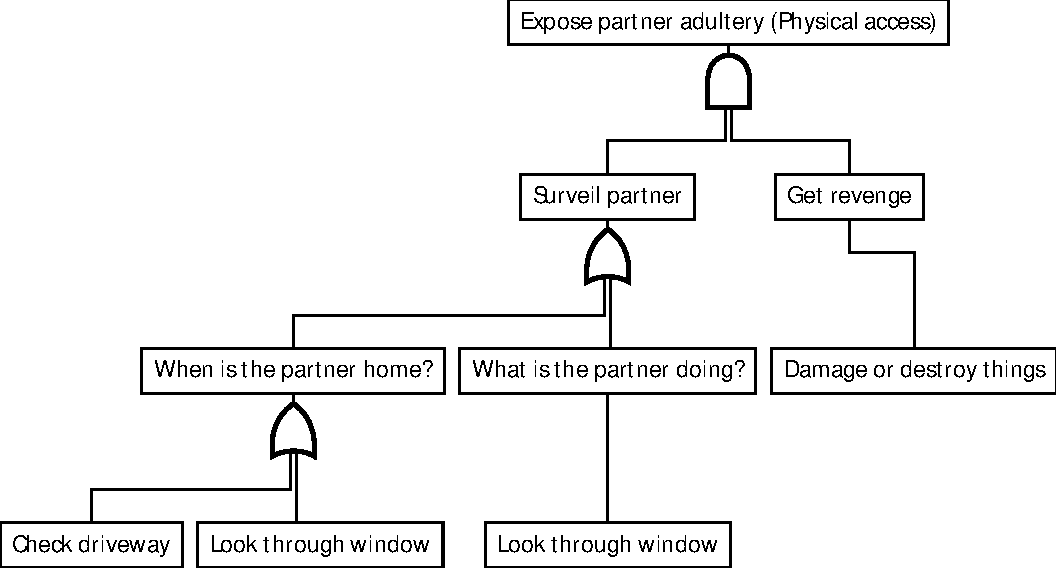
\includegraphics[width=\textwidth]{figures/graphviz/partner_vs_consumer_physical.pdf}
  \caption{The Partner attacking the Consumer by physical means.}
  \label{fig:attack_trees:partner:cheater_physical}
\end{figure}

\begin{figure}[h]
  \centering
  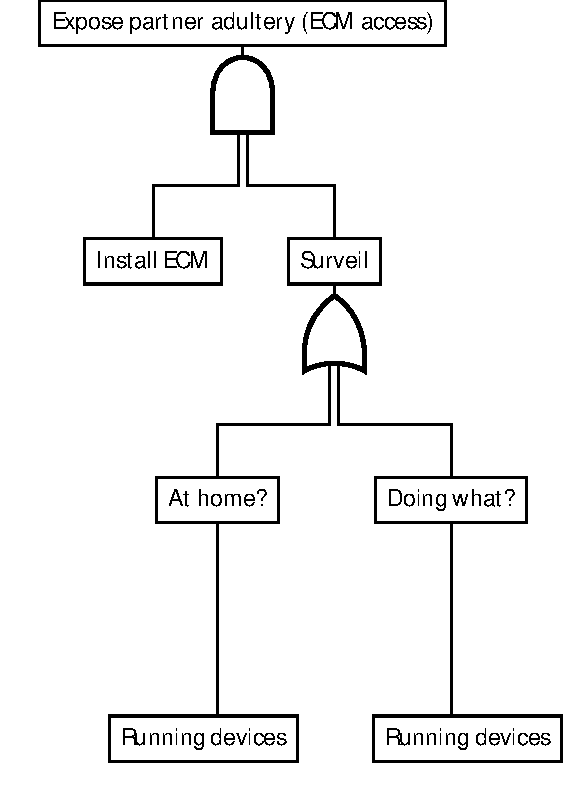
\includegraphics[width=\textwidth]{figures/graphviz/partner_vs_consumer_ecm.pdf}
  \caption{The Partner attacking the Consumer using an ECM.}
  \label{fig:attack_trees:partner:cheater_ecm}
\end{figure}

\afterpage{% Insert after the current page
\cleardoublepage
\thispagestyle{plain}
\KOMAoptions{paper=A3,paper=landscape}
\recalctypearea

\begin{figure}
  \centering
  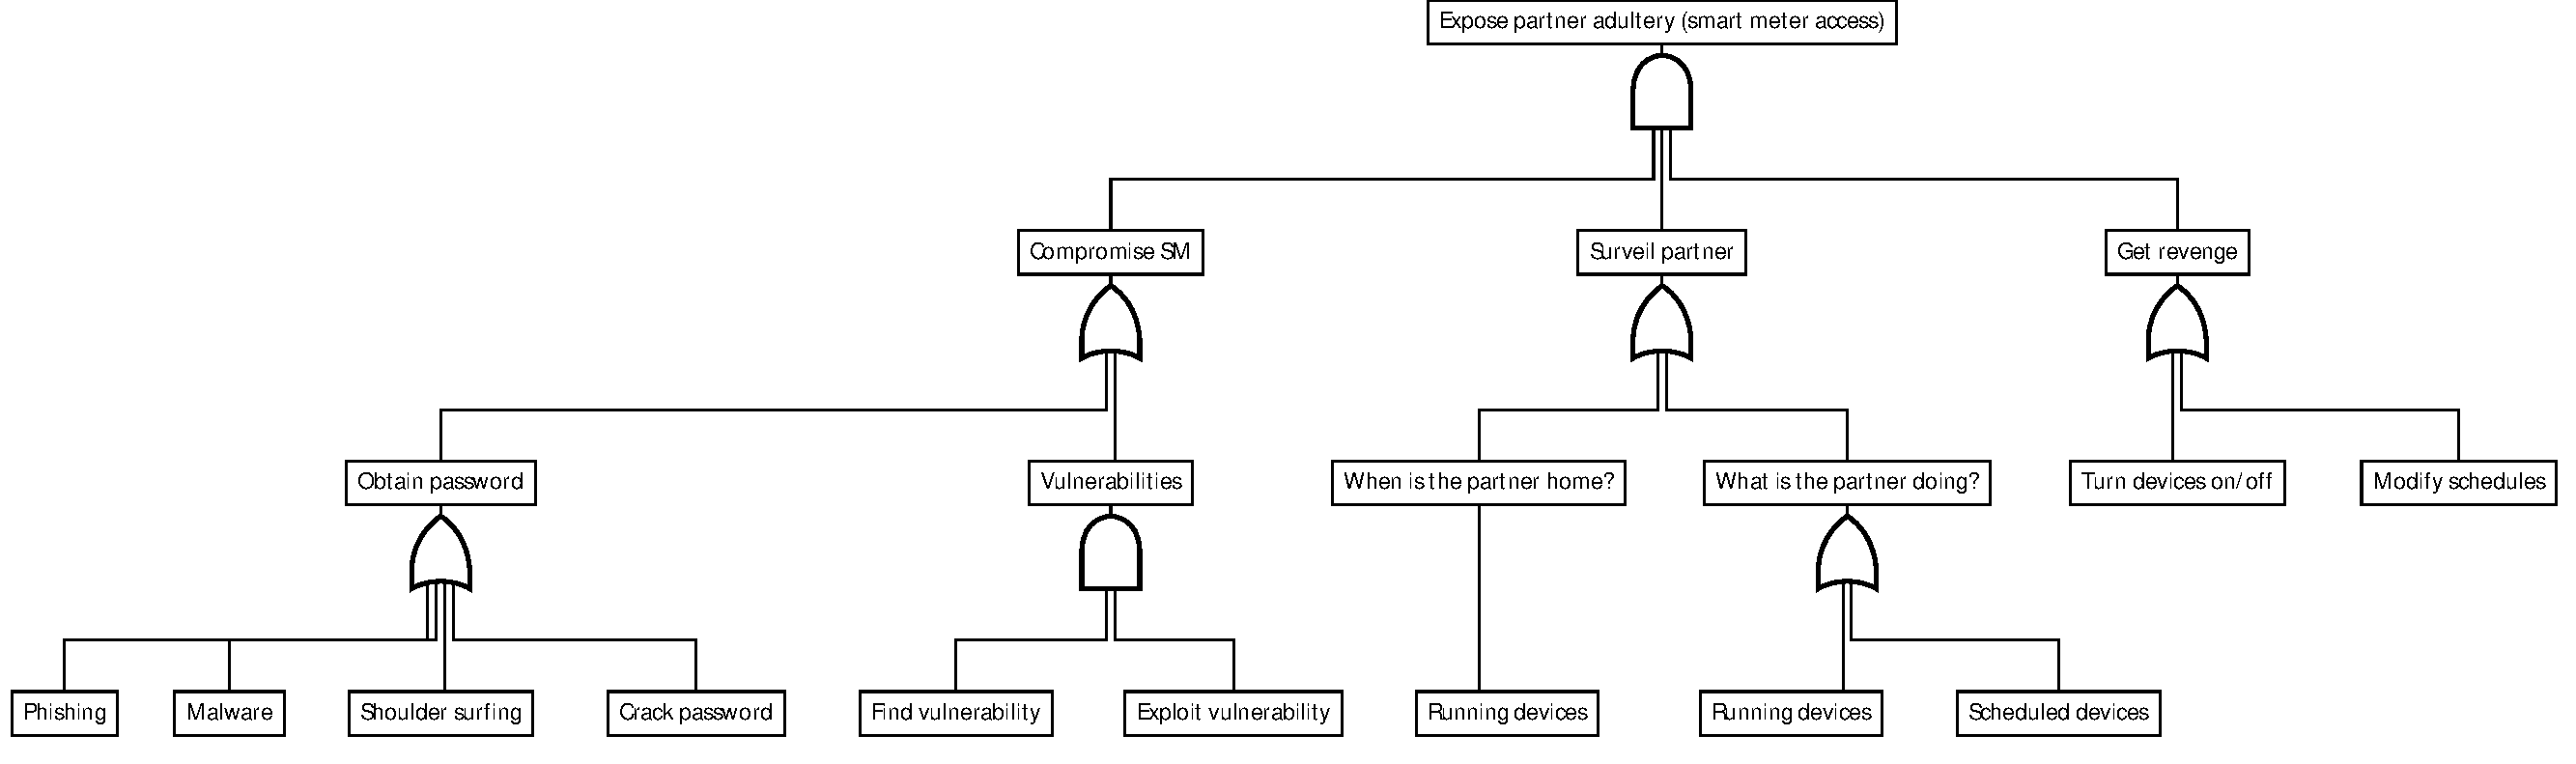
\includegraphics[width=\textwidth]{figures/graphviz/partner_vs_consumer_sm.pdf}
  \caption{The Partner attacking the Consumer by compromising his smart meter.}
  \label{fig:attack_trees:partner:cheater_sm}
\end{figure}

\cleardoublepage
\KOMAoptions{paper=A4,pagesize}
\recalctypearea
}

\begin{figure}
  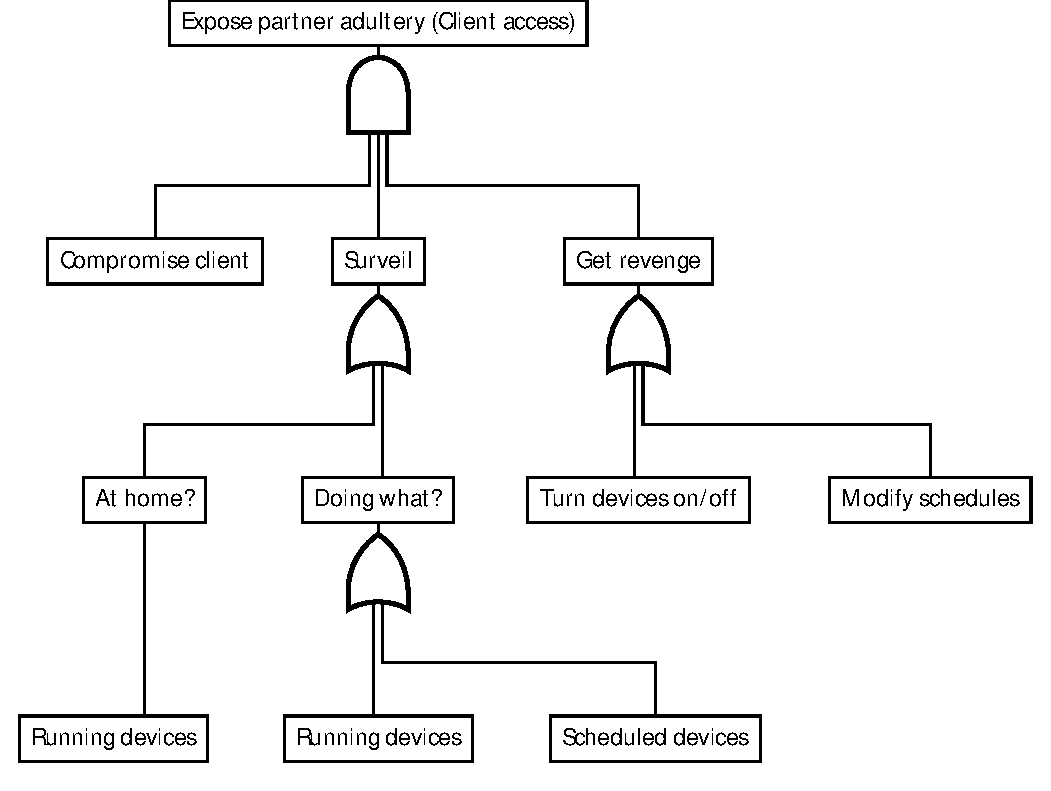
\includegraphics[width=\textwidth]{figures/graphviz/partner_vs_consumer_client.pdf}
  \caption{The Partner attacking the Consumer by compromising his client.}
  \label{fig:attack_trees:partner:cheater_client}
\end{figure}


\subsection{Access}
First of all the partner needs to gain access which can give the partner valuable insight into the doings of the consumer.
In relation to power consumption, the partner has three ways of accessing the consumer's data, which could give the partner the details the partner need to determine whether the consumer is home or not.

\subsubsection{Smart meter}
The first way is to compromise the smart meter.
This variation of the attack is identical to that of the burglar which was described in \cref{compromise:SM}.

\subsubsection{Client}
The other option is to gain access to the client that the consumer uses to control the smart meter.
This variation is similiar to the attack of the burglar described ion \cref{compromise:client}, with the exception that the partner has easier access to the client device.
A situation may arise where the partner has access to the client, and can then copy data from the device.

\subsubsection{ECM}
The partner could install an external consumption monitor\footnote{E.g. a TED (The Energy Detective) used in \cref {smart_meter_privacy}.} on the power grid in the house, giving the partner direct power consumption data.
This attack is similar to the burglar using an ECM described in \cref{compromise:ecm}.
Again the only variation is that the partner is closer to the consumer and therefore has more opportunities for installing the ECM.
For instance the partner could install it directly on the smart meter if the smart meter is hidden in a cupboard in the basement.

\subsection{Surveillance}
The main goal of this attack is to surveil and through this surveillance expose the consumer's misdeeds.
The nodes regarding devices are dependant on gained access through the \textit{Gain access} sub-tree as is represented with individual attack trees based on acquired access.

The partner's initial option is through a physical presence, such as looking through a window.
However, assuming that the partner was able to somehow get hold of the consumer's power consumption data, the partner now has options to expose the consumer from a distance.

First of all, the partner could determine whether the consumer is home, and shouldn't be, or that the consumer isn't home, but should be.
This can be done by looking at which devices are scheduled for tasks or from looking at the device power signatures.
The same method can be used to determine what the consumer is doing if the consumer is home, such as brewing more coffee than usual or taking unusually long showers.
See \cref{smart_meter_privacy} to see how to obtain this information from consumption data.

\subsection{Revenge}
The final step of the attack plan is an optional cold dish of revenge.

The partner could of course destroy stuff by applying physical manipulation in one way or another.
However, if the partner wanted to get creative, the partner could use the previously gained access to the smart meter to manipulate the consumer psychologically.
The partner could turn on/shut off the consumer's appliances at inconvenient times.
If the partner wanted to get even more creative, the partner could modify the appliances' schedules such as turning everything on at late night with low intervals.

%!TEX root = ../master.tex
\section{Information gatherer attacking the consumer}\label{informationGathererVsConsumer}
This section describes the attack tree for people who want to obtain private information about the consumer and use the information to construct a profile of the consumer.
Some of the possible actors that want to obtain information from the consumer are listed below:
\begin{itemize}
\item Commercial company, to better aim advertisements and commercials directly to the consumer
\item Appliance company, aiming advertisements and commercials as well as information about their market share and their competition
\item Intelligence agency, for surveillance
\item The government wanting to monitor their citizens
\end{itemize}

The attack tree can be seen on \cref{information_stealing_tree}.
The overall goal of the information gatherer is to construct a profile of the consumer.
The ``traditional'' way of doing this would be to buy this information from someone who has gathered this information.
This could be other actors from the list mentioned above, like Facebook or Google who continuously get information about its customers.
The introduction of the smart meter into the home of consumers provide a new way of collecting this information.
The sub-tree describing how to profile a customer will be described in the following sections.

\afterpage{% Insert after the current page
\cleardoublepage
\thispagestyle{plain}
\KOMAoptions{paper=A3,paper=landscape}
\recalctypearea

\begin{figure}
  \begin{center}
    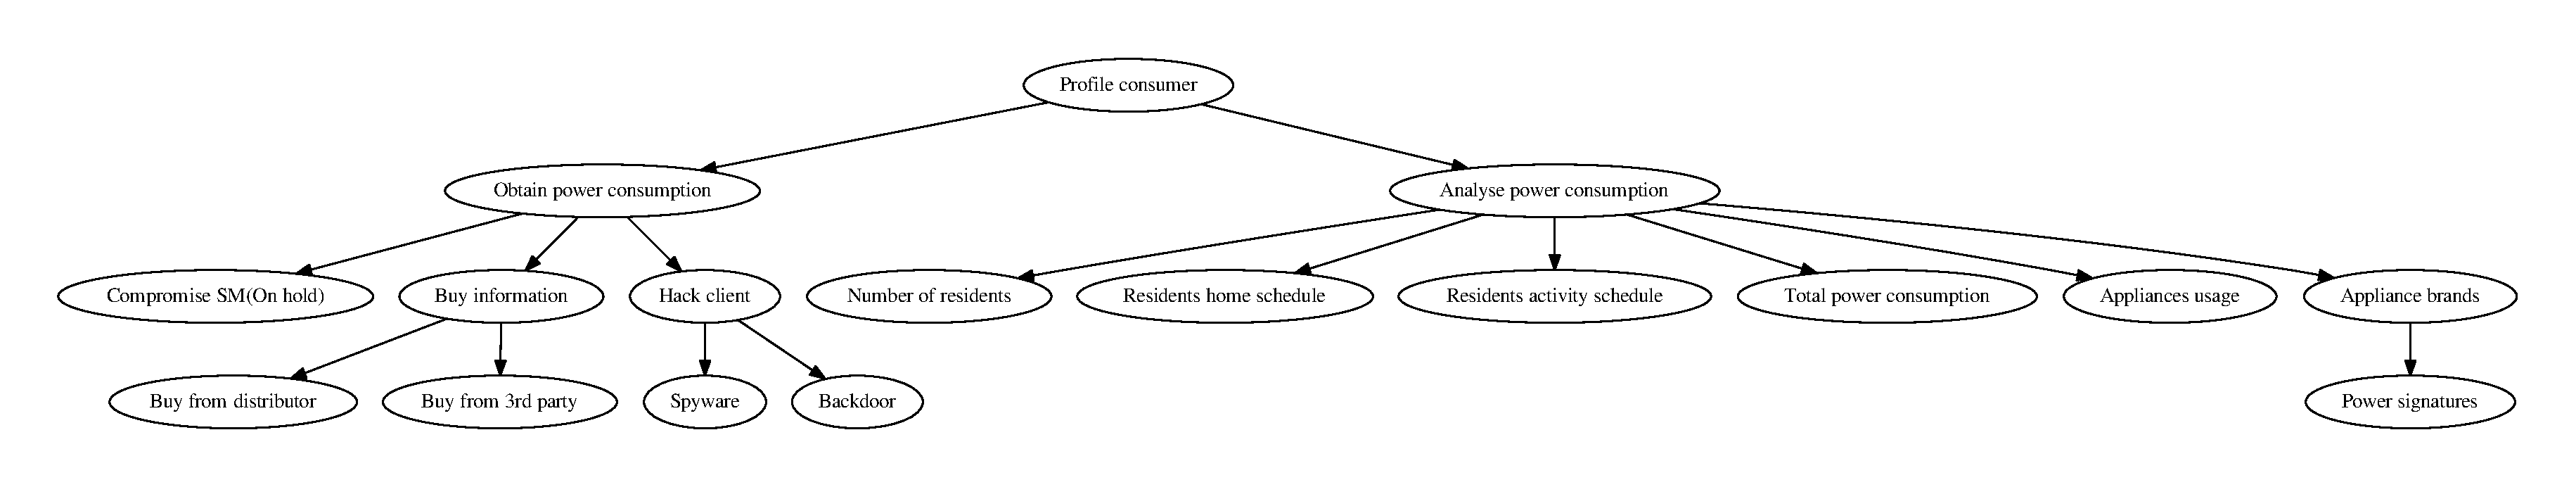
\includegraphics[width=\textwidth]{graphviz/information_stealing_vs_consumer_tree.pdf}
  \end{center}
  \caption{A information gatherer attacking the consumer by stealing his data.}
  \label{information_stealing_tree}
\end{figure}

\cleardoublepage
\KOMAoptions{paper=A4,pagesize}
\recalctypearea
}


\subsection{Obtain power consumption}
In order to analyze the consumption data of the consumer the information gatherer must obtain the consumption first.

\subsubsection{Compromise smart meter}
This subtree is similar to the subtree of the burglar getting access to the smart meter, which was discussed in \cref{compromise:SM}.
The only difference is that \emph{shoulder surfing} is omitted because the information gatherer is further away from the consumer and does not have the opportunity to get close to the consumer.

\subsubsection{Compromise client}
This subtree is similar to that of the burglar described in \cref{compromise:client}.
The only difference is the omission of the \emph{Steal client} option, again because the information gatherer is not in the immediate vicinity of the consumer.

\subsubsection{Buy power consumption}
Another possibility is to buy the information either from someone who has gained access to it or directly from the consumer.
When buying from the consumer social engineering can be used to convince the costumer to sell his data either cheap or against his will.

\subsection{Analyze power consumption}
After gaining access to the smart meter and the consumption data there are many things that can be revealed about the household and the consumers activities and appliances.
See \cref{smart_meter_privacy} to see an example of how the consumption data could be used to reveal this information.


\clearpage

\printbibliography[heading=bibintoc]
\label{bib:mybiblio}
\appendix

\end{document}
